\chapter{Attentive Guidance}\label{Chapter:proposals}

In this chapter I introduce the concept of \textbf{Attentive Guidance (AG)} which is a novel mechanism to equip seq2seq models with an additional bias to nudge them in the direction of finding a compositional solution from the search space of all possible solutions. This chapter begins with a brief overview of the prime motivation for my proposal, followed by the details of attentive guidance. I conclude my discussion on AG by showing how attentive guidance relates to the concept of pondering that we saw in section \ref{mtv:ponder}. This chapter then introduces two datasets which serve as testbeds for attentive guidance. I motivate the relevance of these datasets as pertinent test regimes for attentive guidance followed by the experimental setup for both a vanilla seq2seq baseline and an attentive guidance model. I conclude with the results obtained and a comparative analysis of vanilla seq2seq and attentive guidance on each of these domains.

%(models capable of zero shot generalizing to unseen inputs on known compositions). Additional these small percentage of models also only showed a weak form of composition wherein if for instance t1, t2 are atomic tables, then a composition task t1 t2 is indexed to prompt t1t2, instead of solving in a nested fashion viz. t1(t2(.)). (Get feedback here, see if this is clear)

\section{Attentive Guidance}

\subsection{Inspiration} 

\cite{Lake2015} introduced Hierarchical Bayesian Program Learning (HBPL) to learn complex characters (concepts) from few samples by representing them as probabilistic programs which are built compositionally via. bayesian sampling from simpler primitives, subparts, parts and the relations between them, respectively. This approach led to human level generalization on the \textbf{omniglot} dataset \citep{Lake2015} which is a dataset containing 1623 characters (concepts) with 20 samples each. Omniglot is therefore not sample intensive and hence ideally suited to test one-shot generalization capabilities of a model. This work served as the major motivation for learning nested functions such as \textit{lookup tables} (section \ref{datasets:lt}) of the form t1(t2(.), by learning the compositions from simpler primitives i.e. atomic tables and then stacking them hierarchically. The procedure for learning the \textbf{trace} of the above-mentioned task is described subsequently.

\subsection{Implementation}

Attention (section \ref{mtv:attn}) based seq2seq models produce a \lq soft{}\rq\ alignment between the source (latent representation of the input) and the target. Furthermore seq2seq models require thousands of samples to learn this soft alignment. However in light of the aforementioned arguments presented in favor of concentrating on primitives to construct a complex \lq composition{}\rq\ I propose the concept of \textbf{A}ttentive \textbf{G}uidance (AG). AG argues that the decoder having perfect access to the encoder state(s) containing maximum information pertaining to that decoding step, would leave to improved target sequence accuracy.

%\begin{figure}
%	\begin{minipage}[t]{\textwidth}
%		\ifpdf
%		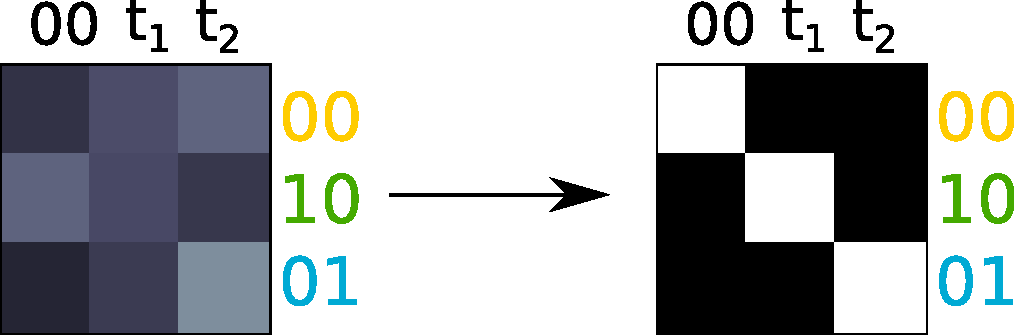
\includegraphics[width=\linewidth,keepaspectratio=true]{./figs/attention-guidance-pdf}
%		\else
%		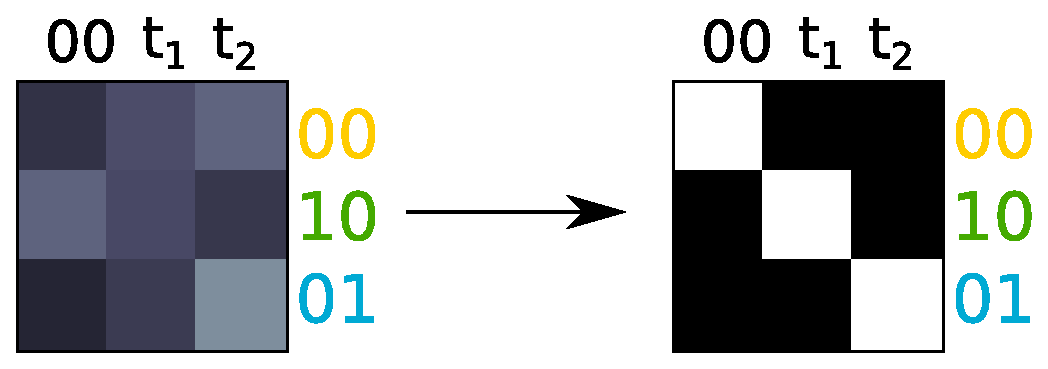
\includegraphics[width=\linewidth,keepaspectratio=true]{./figs/attention-guidance-eps}
%		\fi
%		\caption{\small Diffused vs Hard Attention}
%		\label{pm:ag-schematic}
%	\end{minipage}
%\end{figure}

Revisiting the query-key-value pair view of attention described in section \ref{mtv:attn}, AG tries to improve the scalar matching score between the query and the keys during the attentive read step. Since the \textit{keys} can be thought of as the memory addresses to the \textit{values} which are needed at a given decoding step, AG tries to ensure a more efficient information retrieval. Similar to \cite{Lake2015} AG induces the trace of a program (albeit not probabilistic) needed to solve a complex composition by solving its subparts in a sequential and hierarchical fashion. This in turn forces the model search for a compositional solution from the space of all possible solutions. AG eventually results in a \lq hard{}\rq\ alignment between the source and target.
%as seen in figure \ref{pm:ag-schematic}


\begin{figure}
	\begin{minipage}[t]{\textwidth}
		\ifpdf
		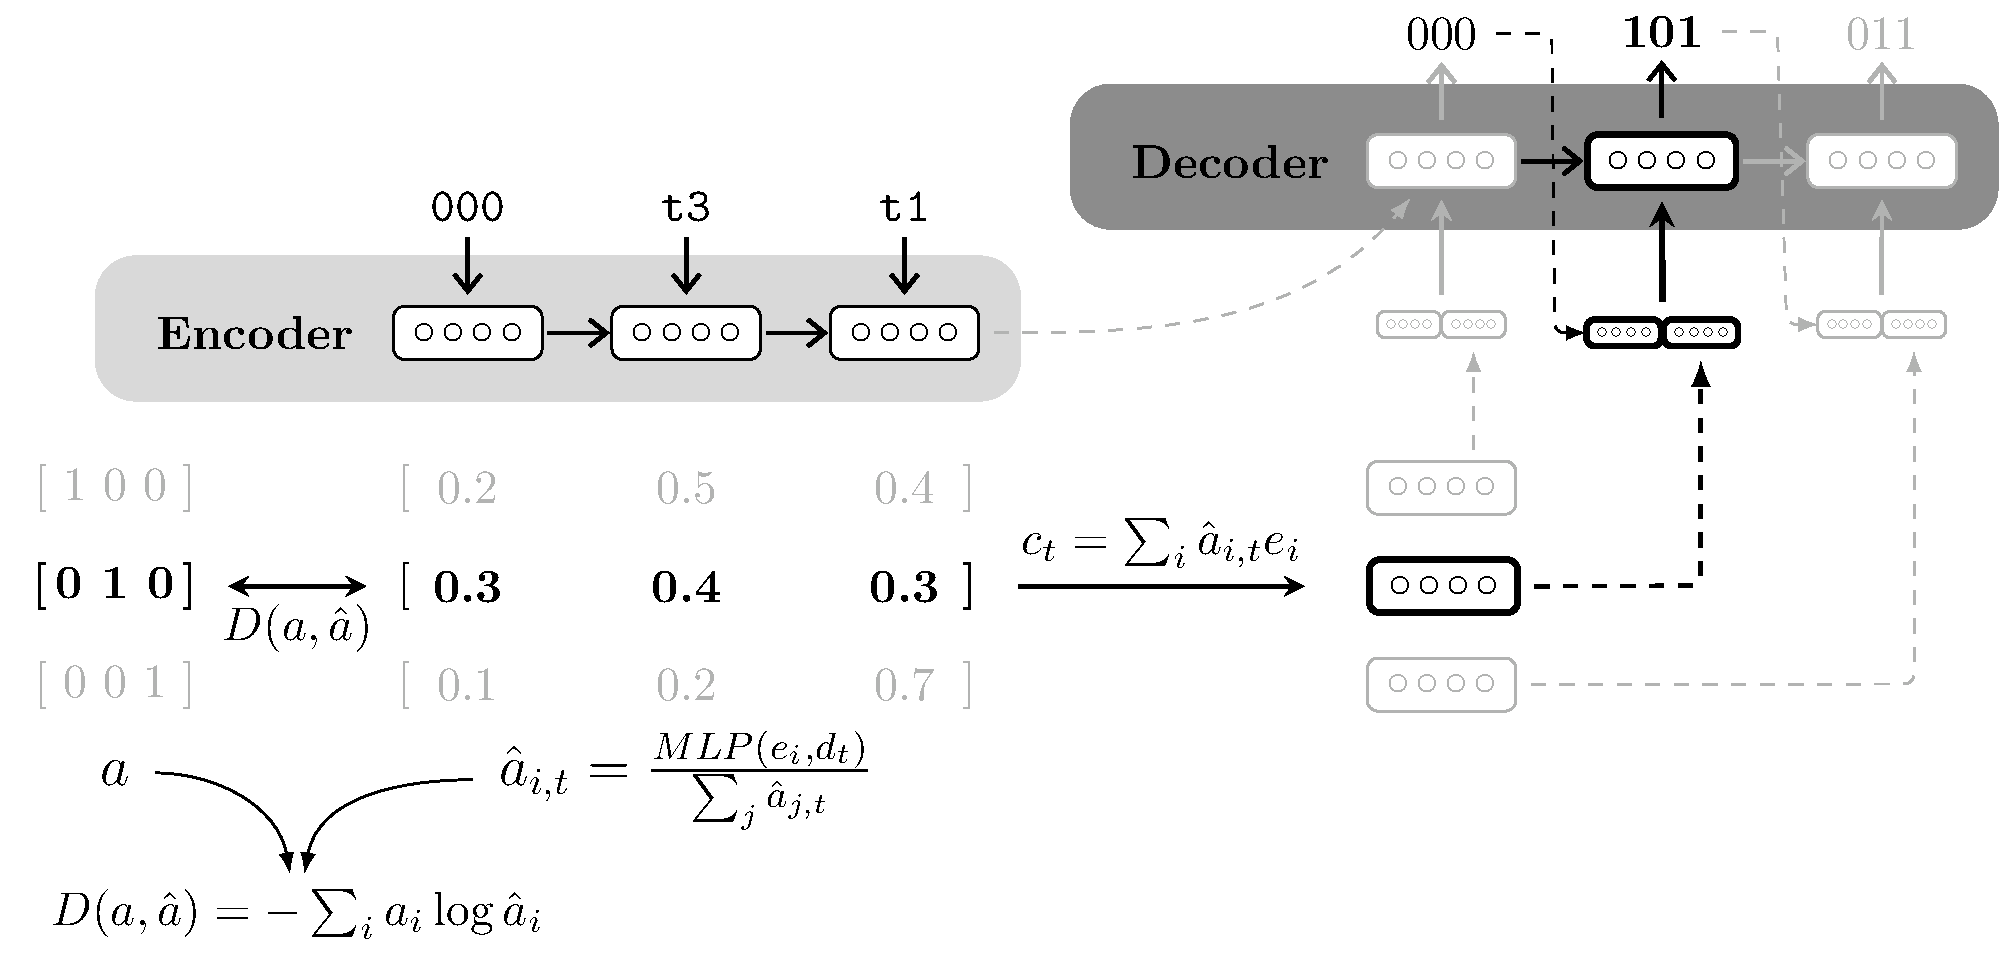
\includegraphics[width=\linewidth,keepaspectratio=true]{./figs/ag-model-pdf}
		\else
		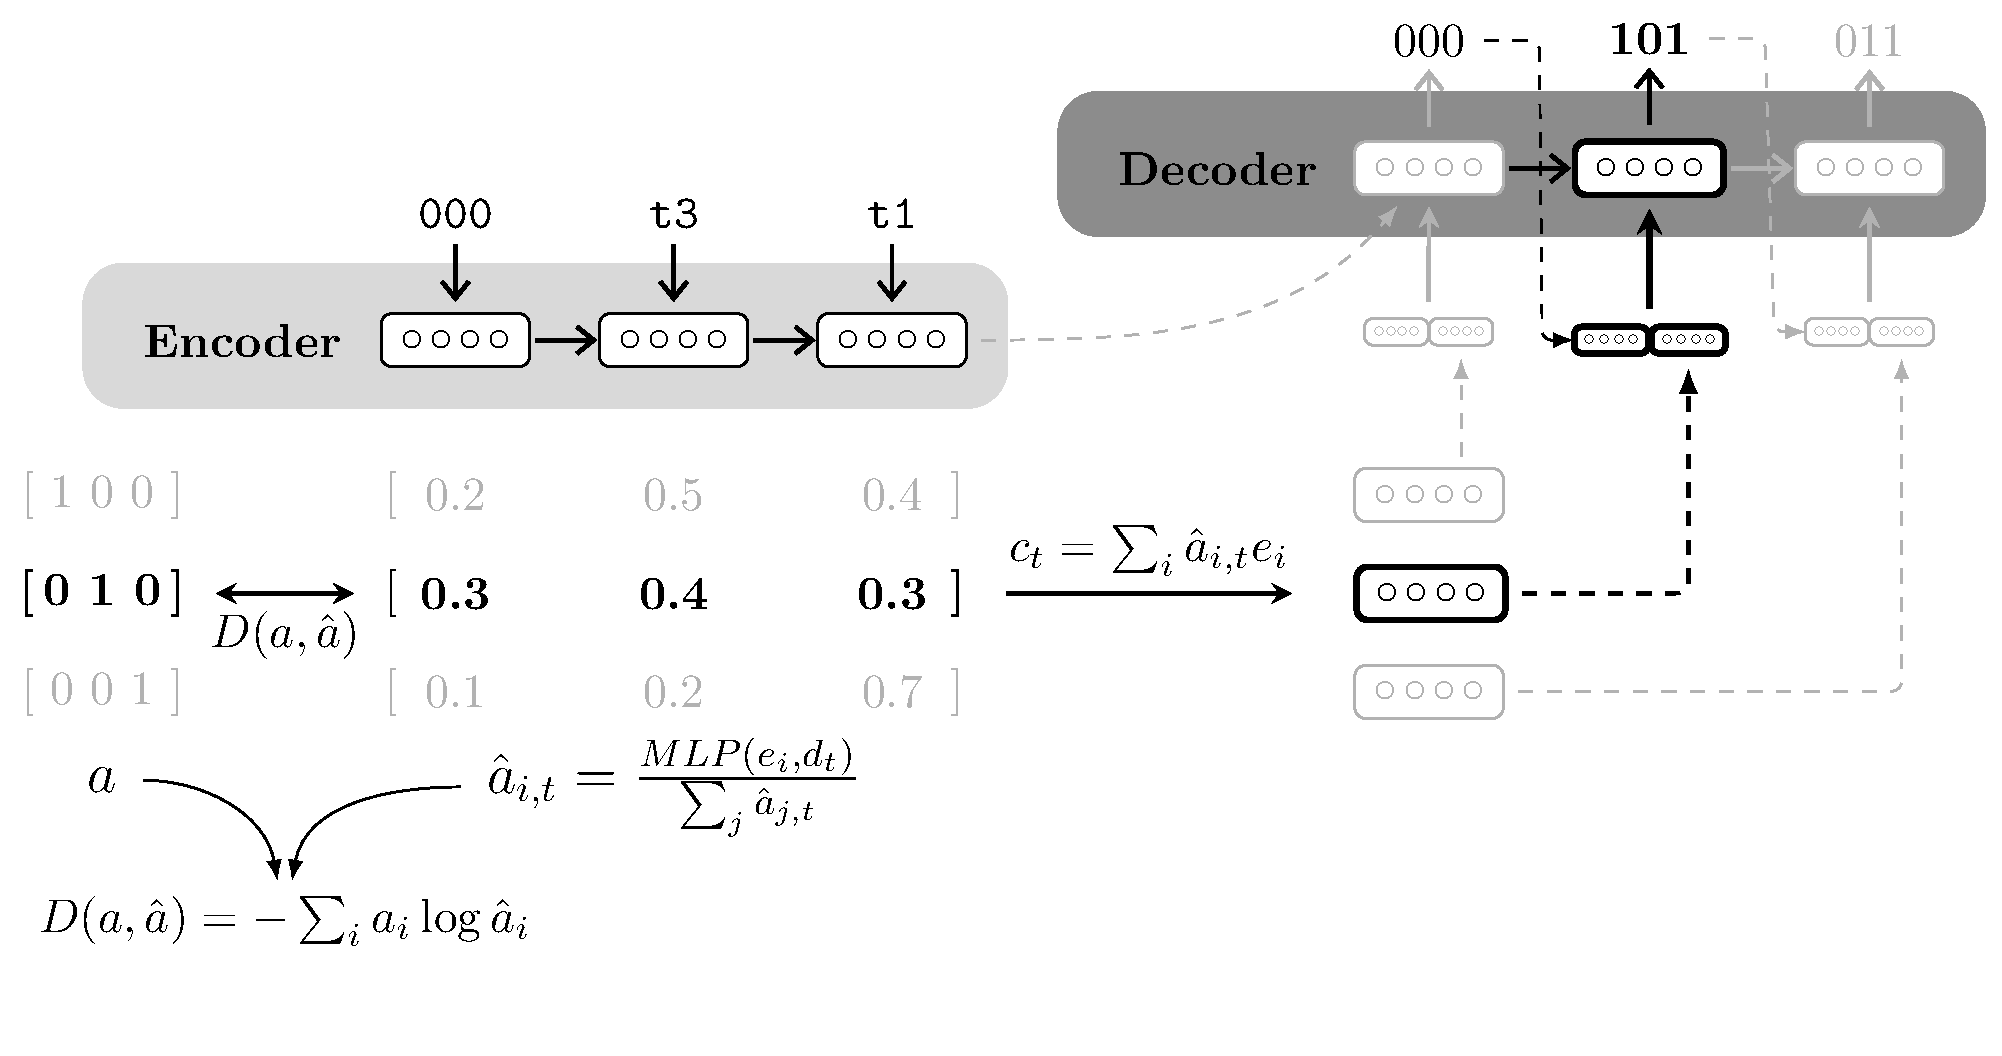
\includegraphics[width=\linewidth,keepaspectratio=true]{./figs/ag-model-eps}
		\fi
		\caption{\small Attentive Guidance and calculation of AG loss \citep{Hupkes2018}}
		\label{pm:ag-loss}
	\end{minipage}
\end{figure}

AG is implemented via an extra loss term added to the final model loss. As shown in figure \ref{pm:ag-loss}, at each step of decoding, the cross entropy loss between calculated attention vector $\hat{a}_{t,i}$ and the ideal attention vector $a_{t,i}$, are added to the model loss. The final loss for an output sequence of length $T$ and an input sequence of length $N$ is therefore expressed as:

\begin{equation}
\widetilde{\mathcal{L}}(x,y) = \mathcal{L}(x,y) + \sum_{t=1}^T \sum_{i=1}^N -a_{i,t}\log\hat{a}_{i,t}
\end{equation}

\subsection{AG and Pondering} \label{pm:ag-ponder}
Pondering presented in section \ref{mtv:ponder} facilitates variable hidden state transitions at any given input step in a recurrent unit. Attentive guidance can be seen as hardcoded or forced pondering in case of seq2seq models. This is best elaborated through an example as follows:
\begin{equation}
	f(5) = 10 \qquad g(3) = 5\qquad f(g(3)) = 10,
\end{equation}
rewriting the composed function as follows and expanding each step of composition:
\begin{equation}
	f\ g\ 3 = 5\ 10.
\end{equation}
It is easy to see that if the above example is presented to a model all it needs to do is emit the final output i.e. 10. However AG forces an additional (ponder) step to explicitly emit the intermediate output as well. Not only does this allow the decoder of the output to have an additional hidden state transition it also helps us see if the model is taking compositional steps in arriving at the final answer. In this thesis we use such \lq mocked\rq{} pondering in case of lookup-tables (section \ref{datasets:lt}) and micro tasks (chapter \ref{Chapter:datasets}). As a future work we can think about coming up with a method to ensure that the number of ponder steps are learned by the decoder instead of being hardcoded.

\section{Lookup Tables} \label{datasets:lt}

The lookup tables task was introduced by \cite{Liska2018} within the CommAI domain \citep{Baroni2017} as an initial benchmark to test the generalization capability of a compositional learner. The data consists of atomic tables which bijectively map three bit inputs to three bit outputs. The compositional task can be understood in the form of a nested function $f(g(x))$ with $f$ and $g$ representing distinct atomic tables. To clarify the task with an example, given $t1$ and $t2$ refer to the first two atomic tables respectively; also given that $t1(001) = 100$ and $t2(100) = 010$. Then a compositional task is presented to a learner as $001 t1 t2 = 010$. Since the i/o strings are three bit, there can be a maximum of 8 input/output strings.

As is very clear from the task description that since the table prompts $t_i$ don't have any semantic meaning in itself, the meaning of each individual table prompt can be correlated only with the bijective mapping it provides. Secondly the dataset is in agreement with the systematic compositionality definition that we have outlined in section \ref{systematic}. Lastly one can argue that even a human learner might come up with an approach that is different than solving each function individually and sequentially in a given nested composition, but such an approach will not be able to scale with the depth of nesting.

\cite{Liska2018} in their experiments with lookup tables found that by having additional supervision on the weights of hidden state transitions, theoretically a finite-state automata (FSA) can be induced such that the recurrent layers encode the states of this automaton. This FSA can in principle solve the lookup table task upto a finite number of compositions. They further showed that this theoretical setup can achieve zero state generalization on unseen inputs on known compositions i.e. \textit{heldout inputs} (section \ref{lt:splits}). However when trained purely on input/output mappings without this additional supervision, the authors noted that only a small percentage of networks could converge to a compositional solution.

%using lookup tables (section \ref{datasets:lt}) as the testbed tried to asses the ability of a RNN network (more specifically a 60 unit LSTM followed by a 10 unit sigmoid layer) to search for compositional solution to the lookup table task. Lookup tables exhibit functional nesting and therefore a model that can find a compositional solution from the search space of all possible solutions is more likely to zero shot generalize to novel compositions. The authors established that

\subsection{Data Structure}\label{lt:splits}
We generated eight distinct atomic tables $t1......t8$ and work with compositions of length two, i.e. $t_i - t_j$. This leads to a possible 64 compositions. Since we want our model to not simply memorize the compositions but rather to land on a compositional solution, we propose to use the compositions only from tables $t1 - t6$ for the training set. However since the model needs to know the mapping produced by tables $t7, t8$ in order to solve their compositions we expose the model to the atomic tables $t7, t8$ in the training set. The details of all the data splits and some dataset statistics are presented below. Examples from each split and the size of each split are presented in table \ref{lt:stats}

\begin{enumerate}
	\item \textbf{train} - The training set consists of the 8 atomic tables on all 8 possible inputs. The total compositions of tables $t1 - t6 = 36$. Out of those 36 compositions we take out 8 compositions randomly. For the remaining 28 compositions we take out 2 inputs such that the training set remains balanced w.r.t. the compositions as well as the output strings. (Details of this sudoku algorithm in the appendix)
	\item \textbf{heldout inputs} - The 2 inputs taken out from the 28 compositions in training constitute this test set. However of the 56 data points, 16 are taken out to form a validation set. In creating this split we ensure that the splits i.e. \textit{heldout inputs} and \textit{validation} have a uniform distribution in terms of output strings at the expense of the uniformity in the compositions.
	\item \textbf{heldout compositions} - This set is formed by the 8 compositions that were taken out of the initial 36 compositions. These 8 compositions are exposed to all 8 possible input strings.
	\item \textbf{heldout tables} - This test is a hybrid of the tables which are seen in compositions during training i.e. $t1 - t6$ and those which are seen just atomically during training i.e. $t7 - t8$. There are total of 24 compositions in this split which are exposed to all 8 inputs.
	\item \textbf{new compositions} - This split consists of compositions of $t7 - t8$ and therefore a total of 4 compositions on 8 inputs.
\end{enumerate}


\begin{table}[ht]
	\centering
	\begin{tabular}{l|lc}
		& Example & Size\\
		\hline
		train & t1 t2 011 & 232 \\
		heldout inputs & t1 t2 001 & 40 \\
		heldout compositions & t1 t3 110 & 64 \\
		heldout tables & t1 t8 111 & 192 \\
		new compositions & t7 t8 101 & 32 \\
	\end{tabular}
	\caption{Lookup Table Splits}
	\label{lt:stats}
\end{table}


\begin{figure}[ht]
	\begin{subfigure}{0.5\linewidth}
		\ifpdf
		\includegraphics[width=0.95\linewidth]{./figs/lookup/train-pdf}
		\else
		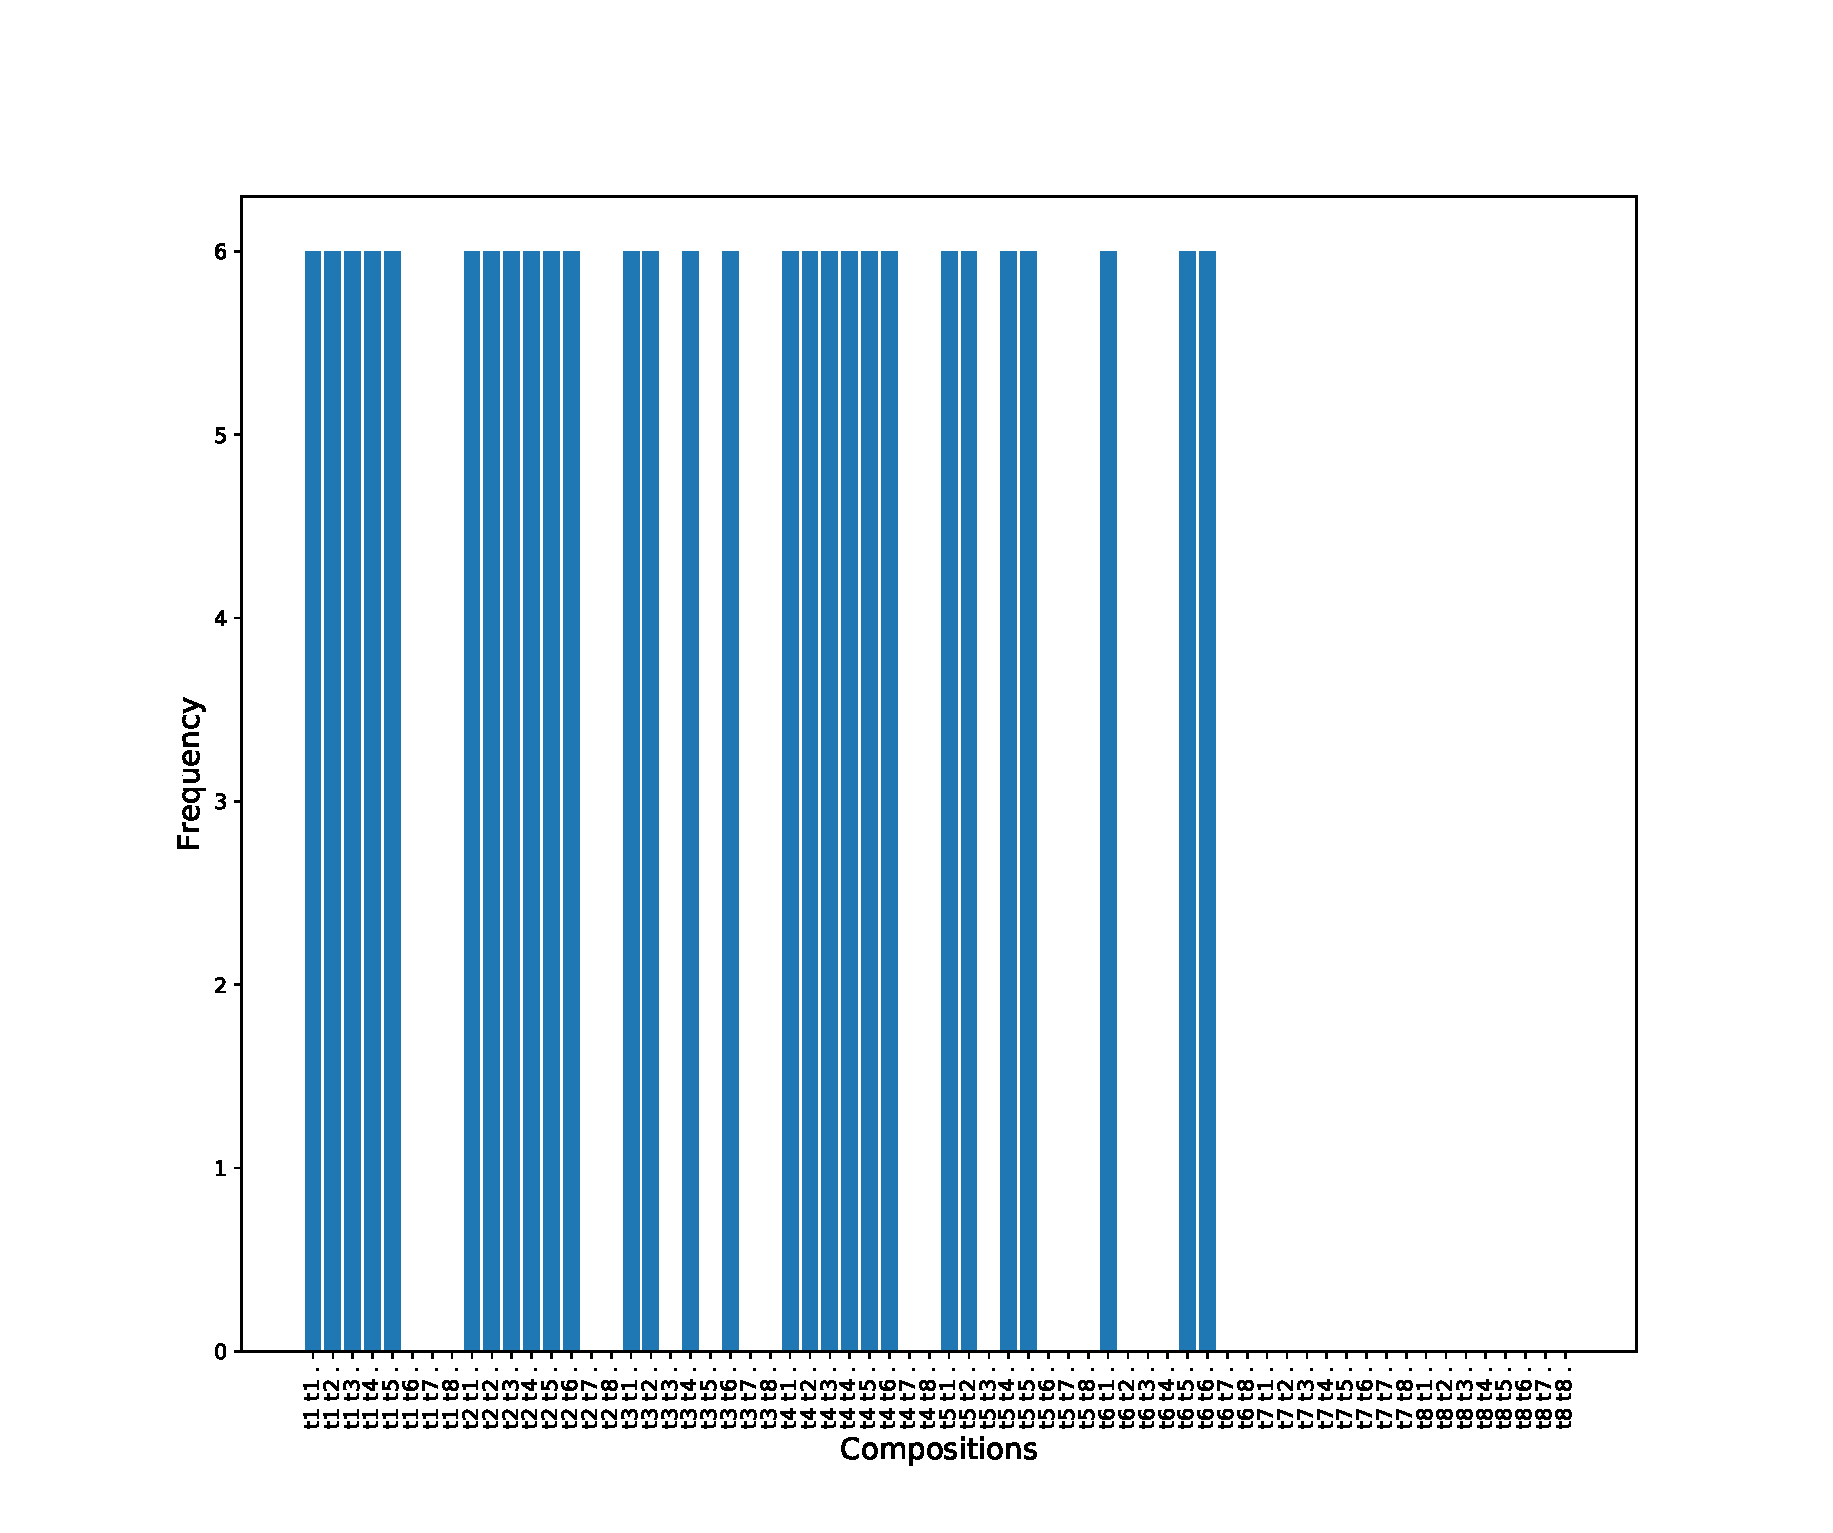
\includegraphics[width=0.95\linewidth]{./figs/lookup/train-eps}
		\fi
		\caption{Train}\label{fig:train_dist}
	\end{subfigure}
	\begin{subfigure}{0.5\linewidth}
		\ifpdf
		\includegraphics[width=0.95\linewidth]{./figs/lookup/heldout_compositions-pdf}
		\else
		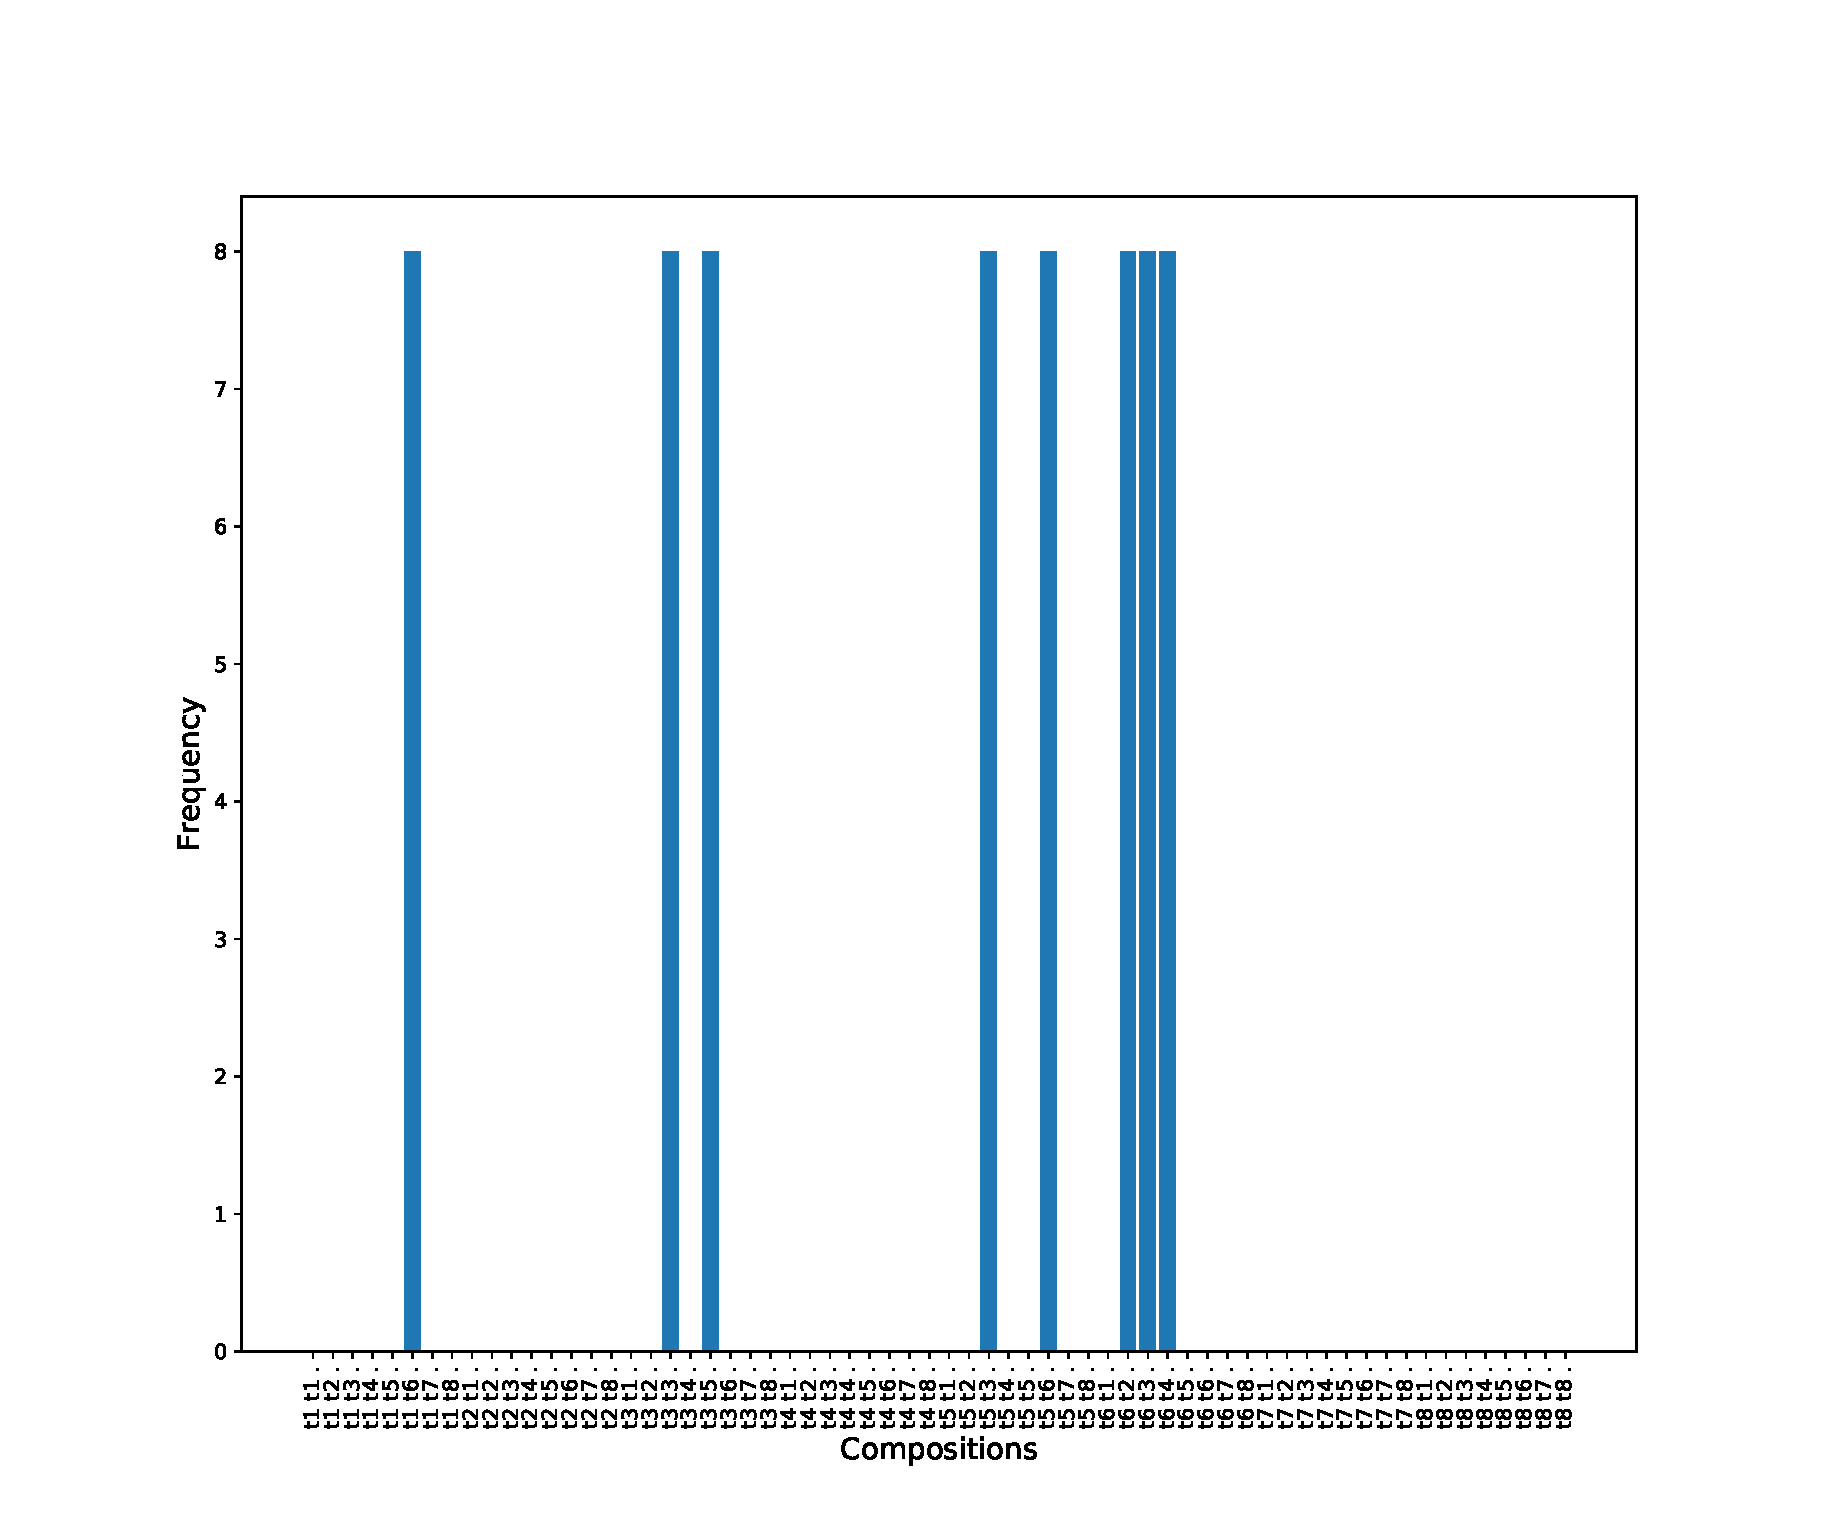
\includegraphics[width=0.95\linewidth]{./figs/lookup/heldout_compositions-eps}
		\fi
		\caption{Heldout Compositions}\label{fig:held_comp}
	\end{subfigure}
	\begin{subfigure}{0.5\linewidth}
		\ifpdf
		\includegraphics[width=0.95\linewidth]{./figs/lookup/heldout_tables-pdf}
		\else
		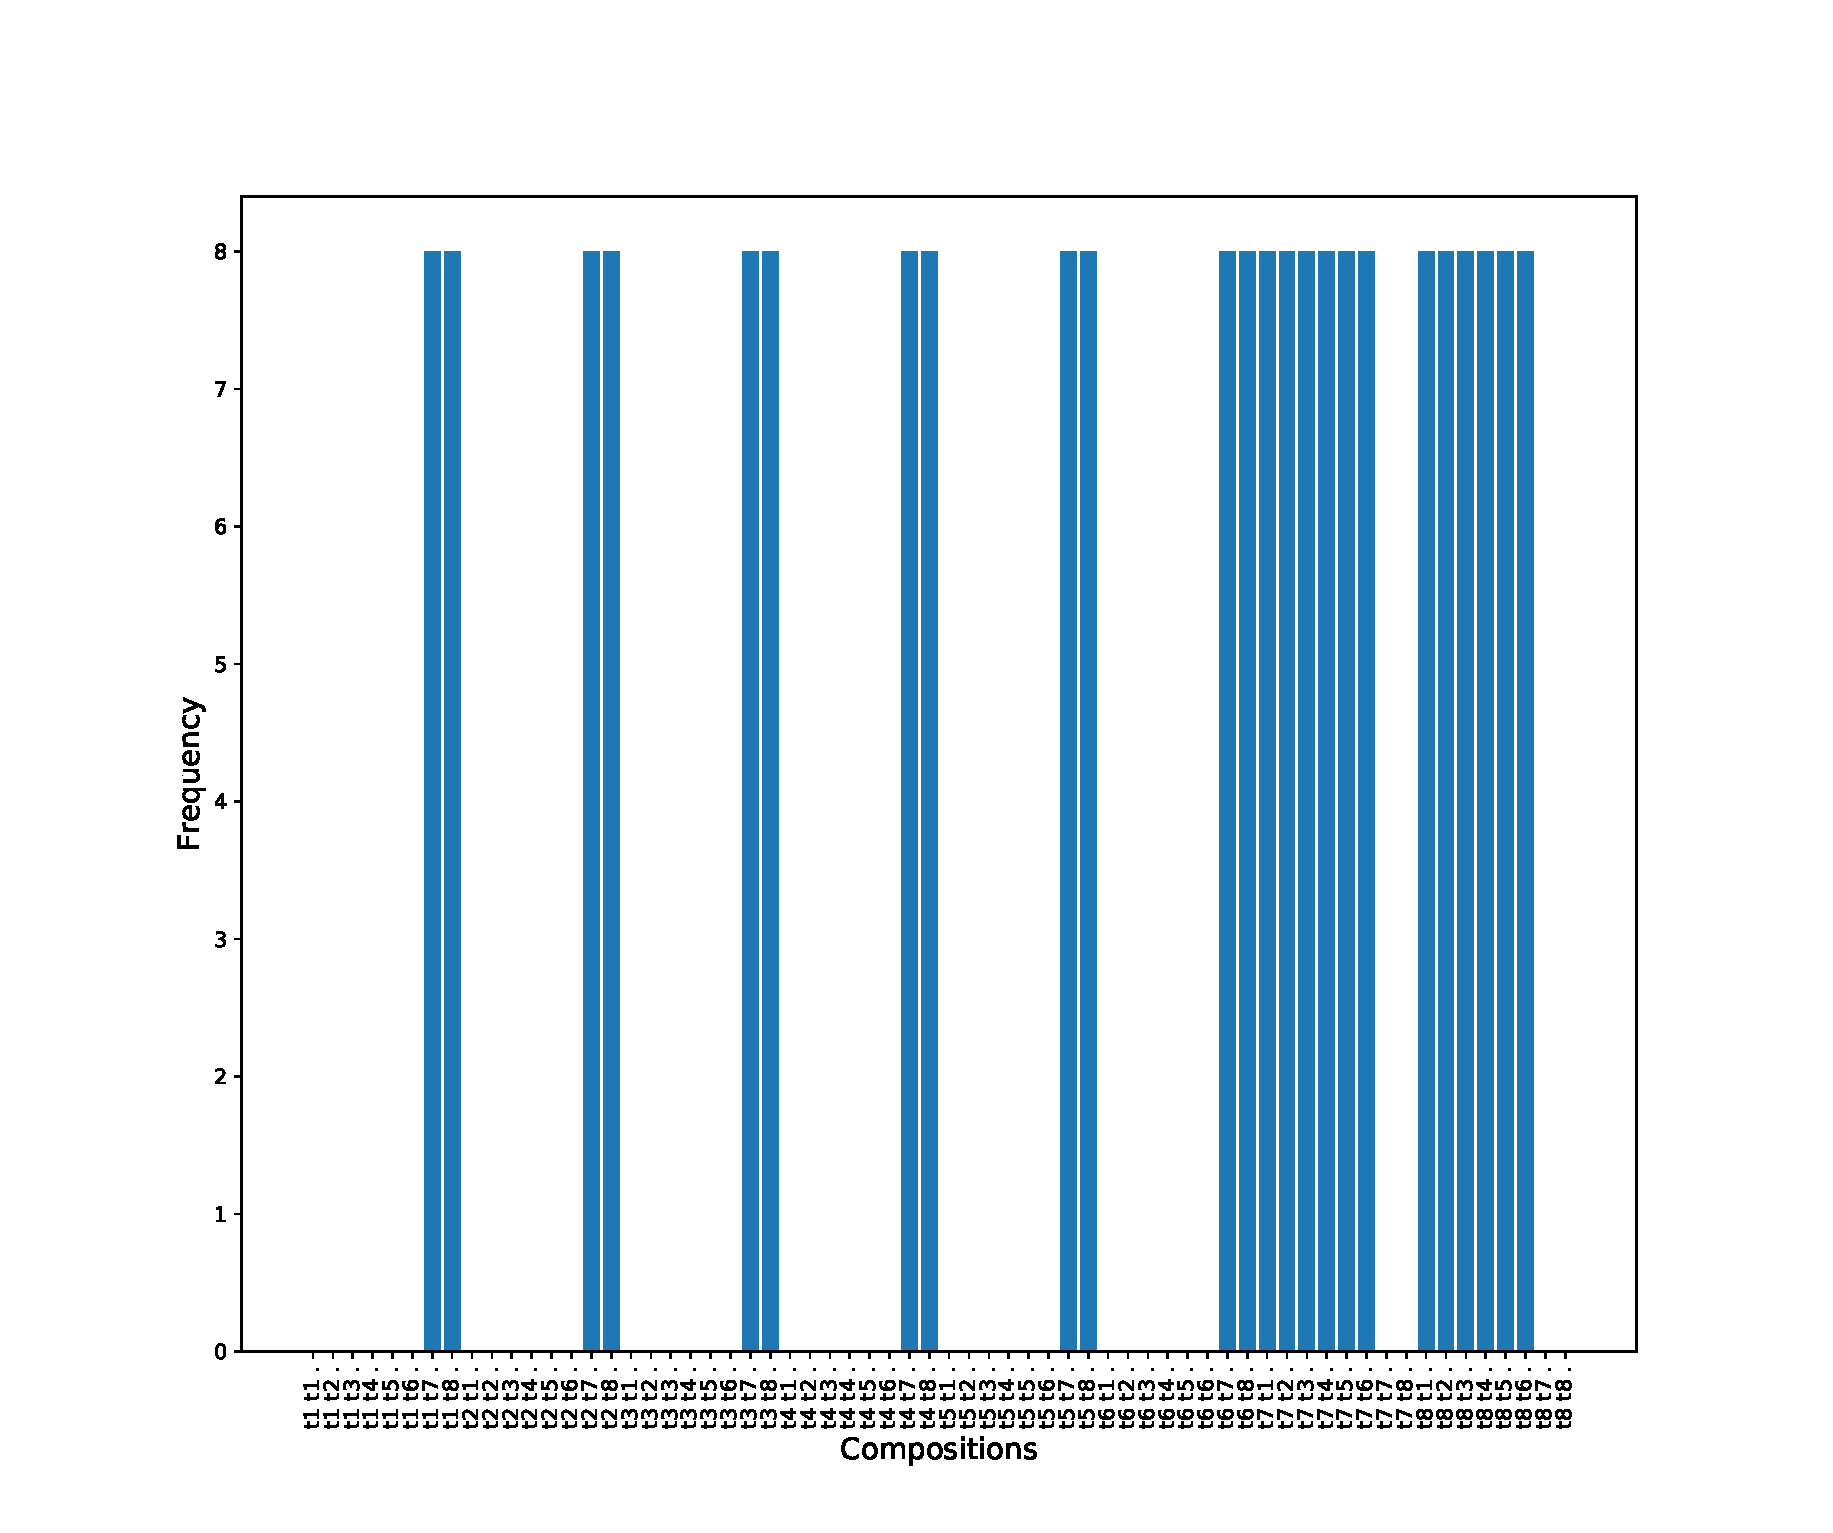
\includegraphics[width=0.95\linewidth]{./figs/lookup/heldout_tables-eps}
		\fi
		\caption{Heldout Tables}\label{fig:held_tab}
	\end{subfigure}
	\begin{subfigure}{0.5\linewidth}
		\ifpdf
		\includegraphics[width=0.95\linewidth]{./figs/lookup/new_compositions-pdf}
		\else
		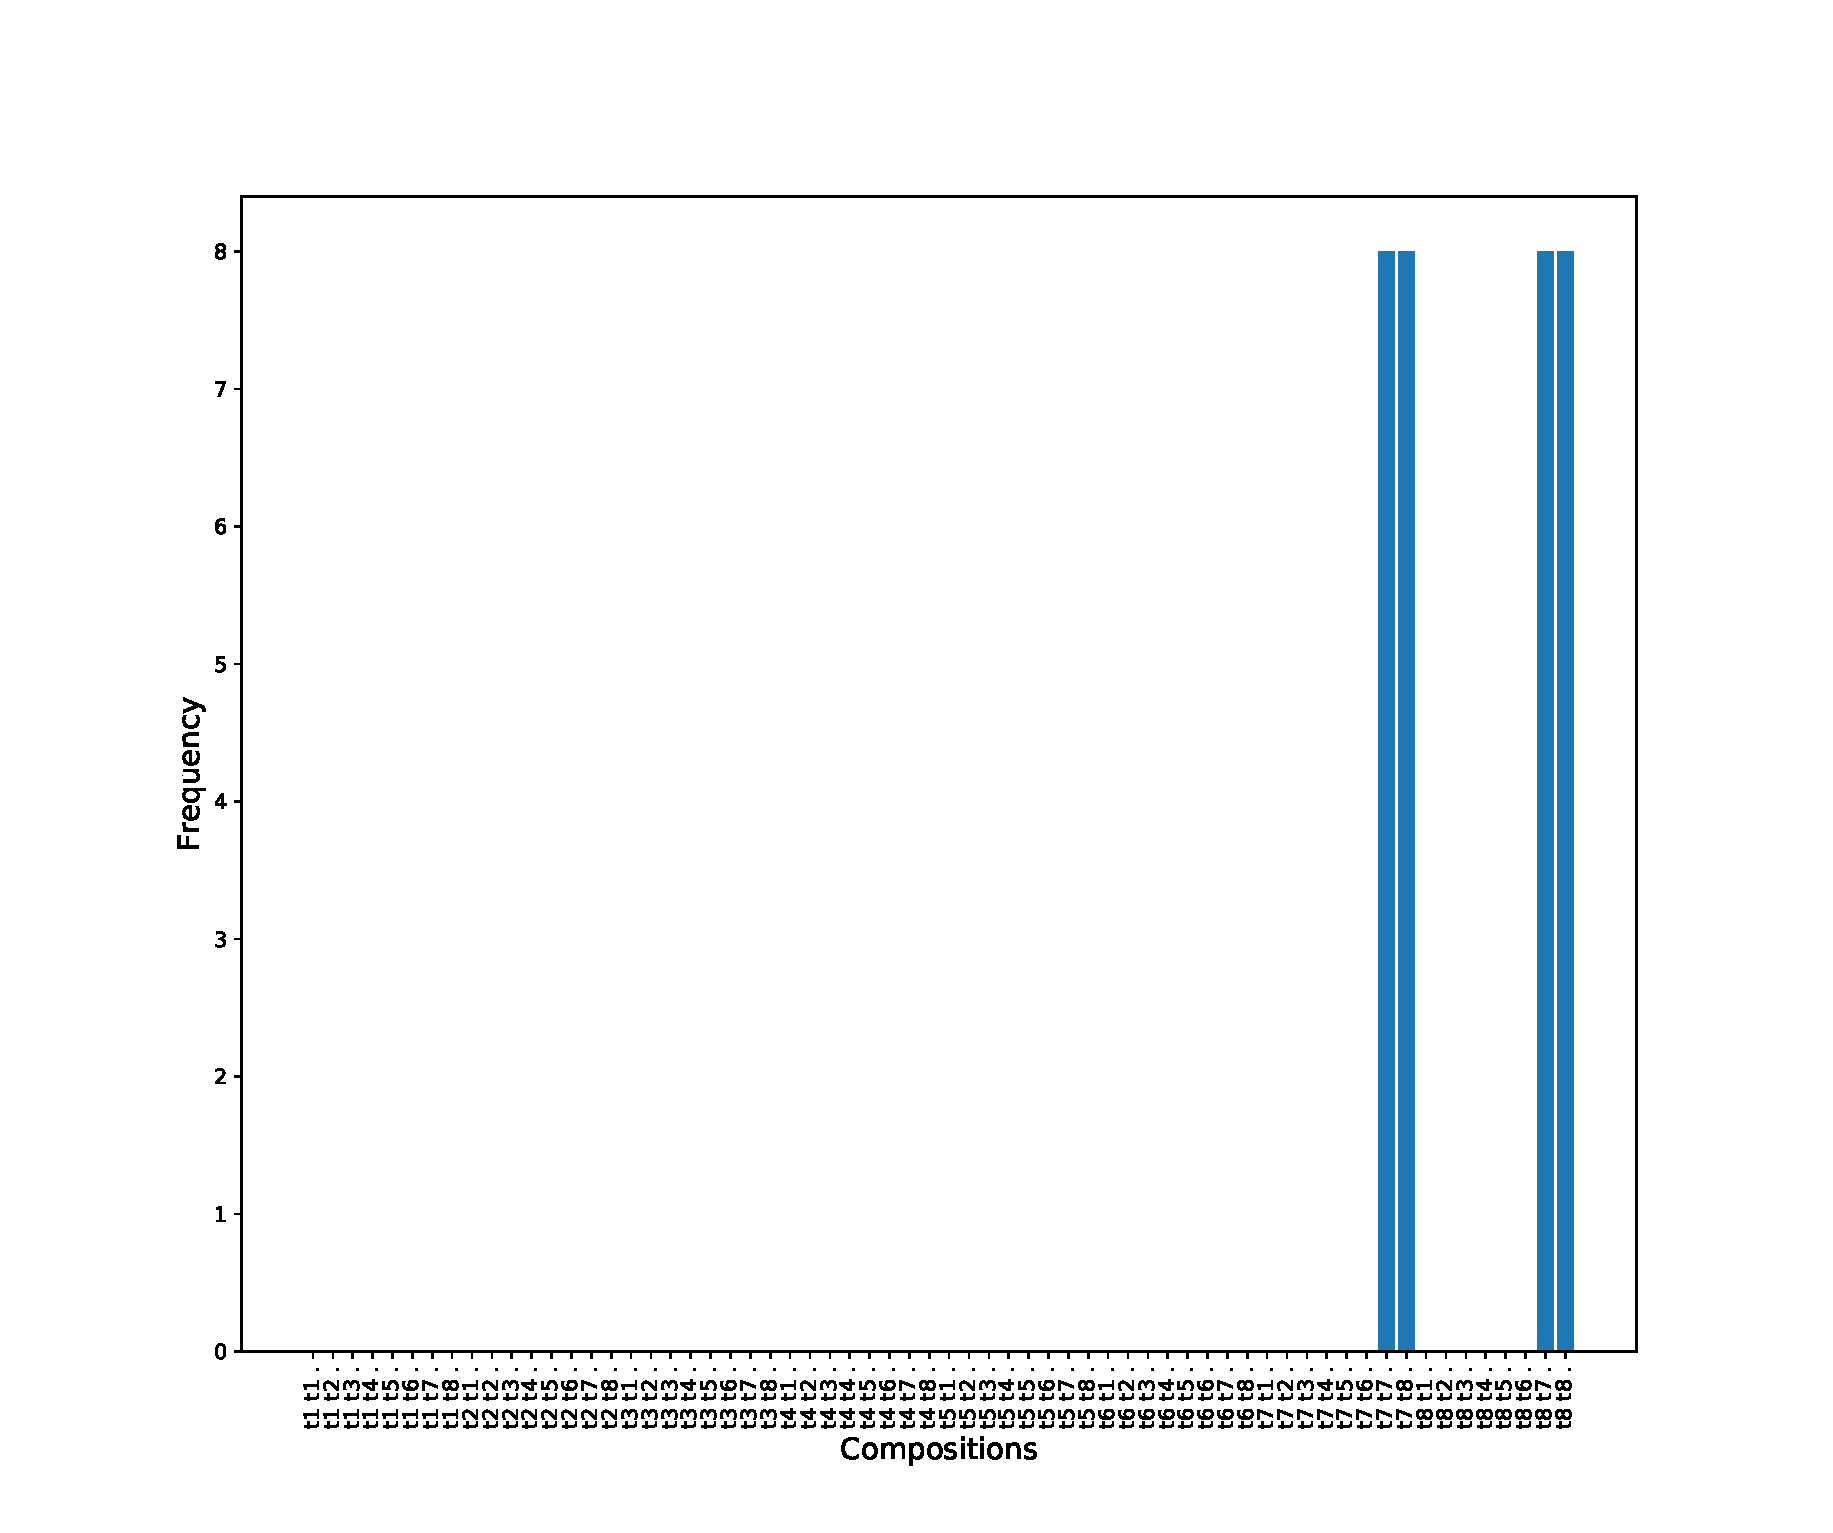
\includegraphics[width=0.95\linewidth]{./figs/lookup/new_compositions-eps}
		\fi
		\caption{New Compositions}\label{fig:new_comp}
	\end{subfigure}
	\caption{Data distribution of train and test sets}\label{fig:all_data}
\end{figure}
%, trim={15mm, 5mm, 35mm, 15mm}, clip
In accordance with the data split described above we present the distribution of all compositions in the train and various test sets. It can be seen that the test sets \lq heldout\_tables\rq{} and \lq new\_compositions \rq{} are the most difficult and require zero-shot generalisation owing to their significantly different distribution as compared to \lq train \rq{}.

\subsection{AG Trace}
As explained in section \ref{pm:ag-ponder} attentive guidance can help in mocking the pondering. For a lookup table composition of the form \lq $((000)t3)t1$ AG enforces pondering as follows:
\begin{equation}
t1(111) = 100 \qquad t3(000) = 111 \qquad ((000)t3)t1 = 100,
\end{equation}
the composed function is expanded as follows:
\begin{equation}
000\ t3\ t1 = 000\ 111\ 100.
\end{equation}
AG therefore forces the decoder to ponder for two additional steps. The biggest difference from the Pondering in section \ref{mtv:ponder} would be that at each pondering step we have an emission, instead of the ponder step being a silent one. The trace for the attentive guidance can be explained as follows:
%and is shown in figure \ref{ag_lt}:
\begin{itemize}
	\item The first step is the copy step where the three bit input to the composition is copies as if.
	\item After this the tables in the composition are applied sequentially to the three bit input preceding them.
	\item The diagonal trace is mean to capture this sequential and compositional solution of lookup tables. At each step of decoding we force the model to focus on only that input prompt which results in the correct output for that step.
\end{itemize}


%\begin{figure}[ht] 
%	\begin{subfigure}[b]{0.5\linewidth}
%		\centering
%		\ifpdf
%		\includegraphics[width=0.95\linewidth]{./figs/lookup/lt-trace-pdf}
%		\else
%		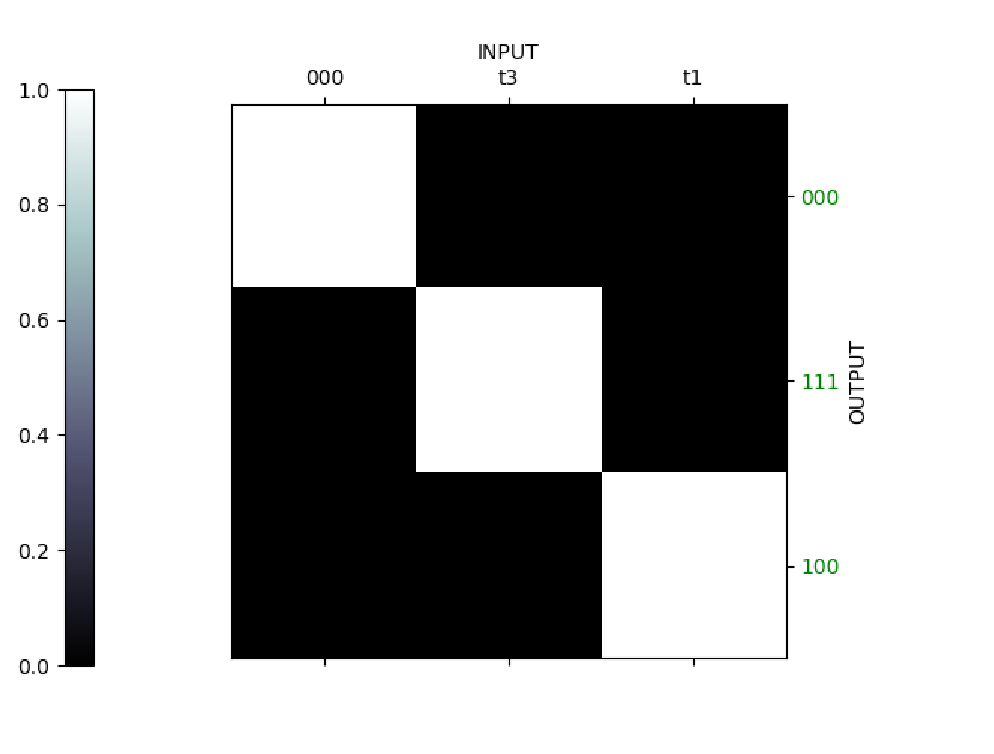
\includegraphics[width=0.95\linewidth]{./figs/lookup/lt-trace-eps}
%		\fi
%		\caption{AG Trace for Lookup Tables} 
%		\label{ag_lt} 
%		\vspace{2ex}
%	\end{subfigure}%% 
%	\begin{subfigure}[b]{0.5\linewidth}
%		\centering
%		\ifpdf
%		\includegraphics[width=0.95\linewidth]{./figs/lookup/sr-trace-pdf}
%		\else
%		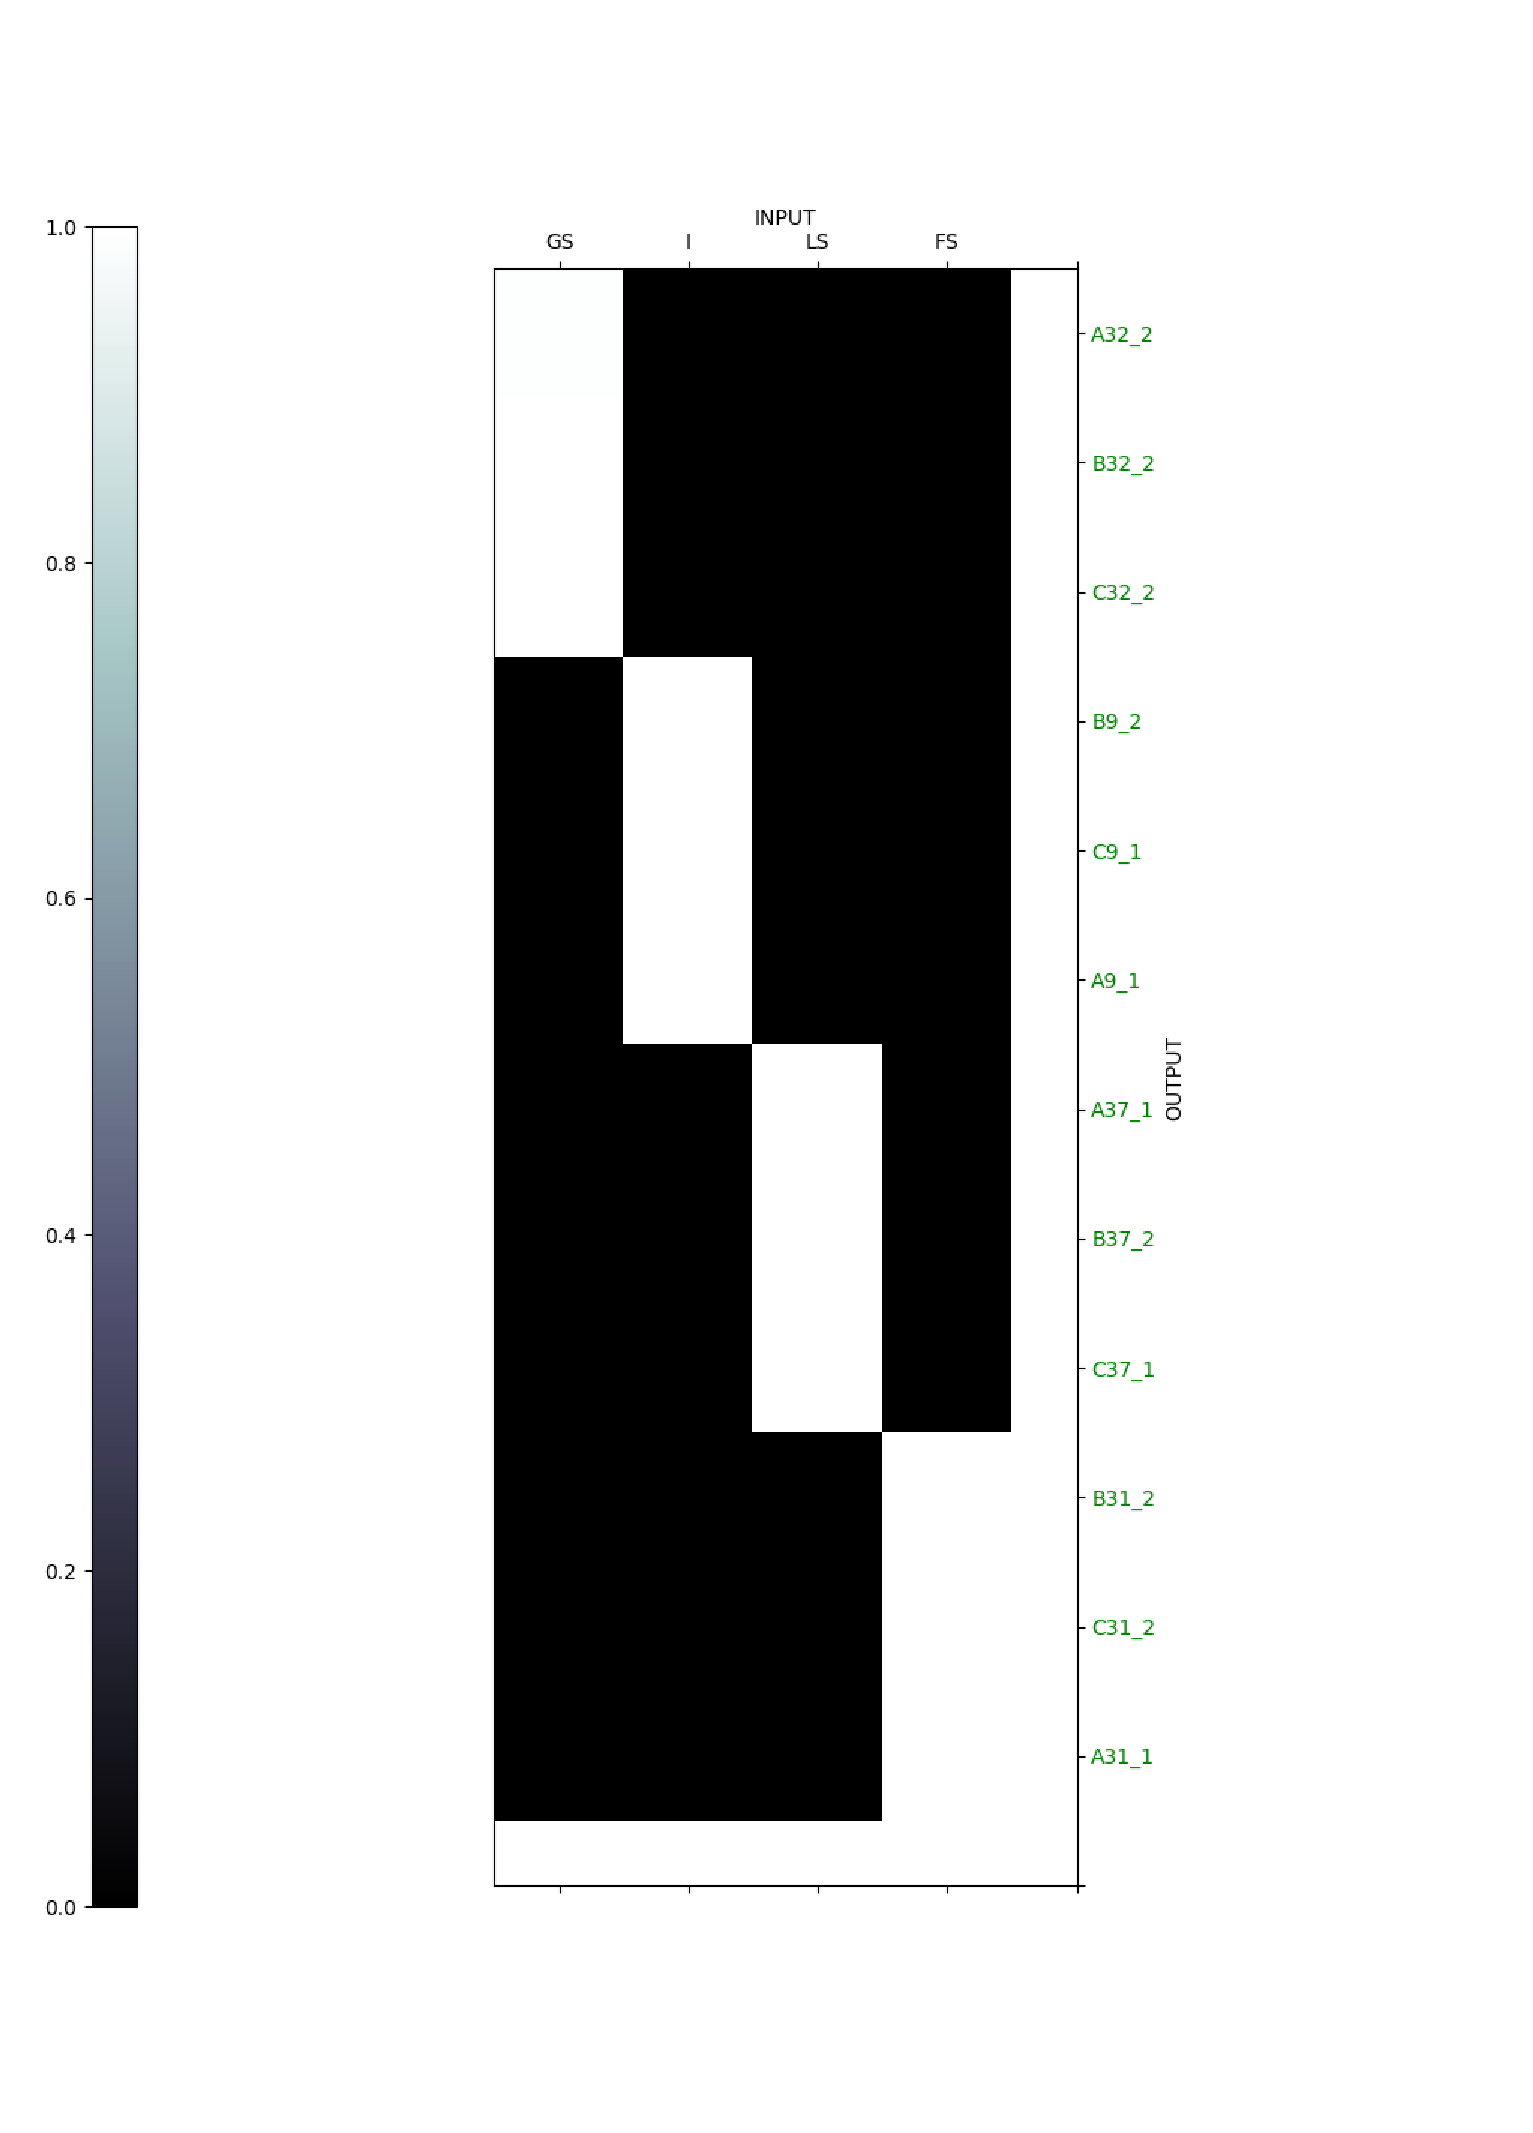
\includegraphics[width=0.95\linewidth]{./figs/lookup/sr-trace-eps}
%		\fi 
%		\caption{AG Trace for Symbol rewriting} 
%		\label{ag_sr} 
%		\vspace{2ex}
%	\end{subfigure}
%	\label{ag_trace_lt_sr}
%\end{figure}


\subsection{Accuracy}
Since the lookup tables can be viewed as nested functions, accuracy of final output of the composition can be an adequate measure of model performance. However since we want to ensure that the model doesn't learn spurious patterns in data to land at an un-compositional solution, we want it to be accurate at each step of the composition. This hierarchical measure of accuracy is a viable test for the compositionality of the network. Therefore in all evaluations \textit{sequence accuracy} is the performance metric of the model.

\subparagraph{Hyperparameters}: Based on the hyperparameter grid search conducted by \cite{Hupkes2018} I ran the experiments with the best hyperparameters for both baseline (RNN cell=GRU, Embedding size=128, Hidden layer size=512, optimizer=Adam \citep{KingmaB14}, learning rate=0.001, attention=pre-rnn \citep{Bahdanau2014}, alignment measure=mlp(section \ref{mtv:attn})).

\subsection{Lookup Tables - Results}
\begin{figure}[ht] 
	\begin{subfigure}[b]{0.5\linewidth}
		\centering
		\ifpdf
		\includegraphics[width=0.95\linewidth]{./figs/lookup/baseline-loss-pdf}
		\else
		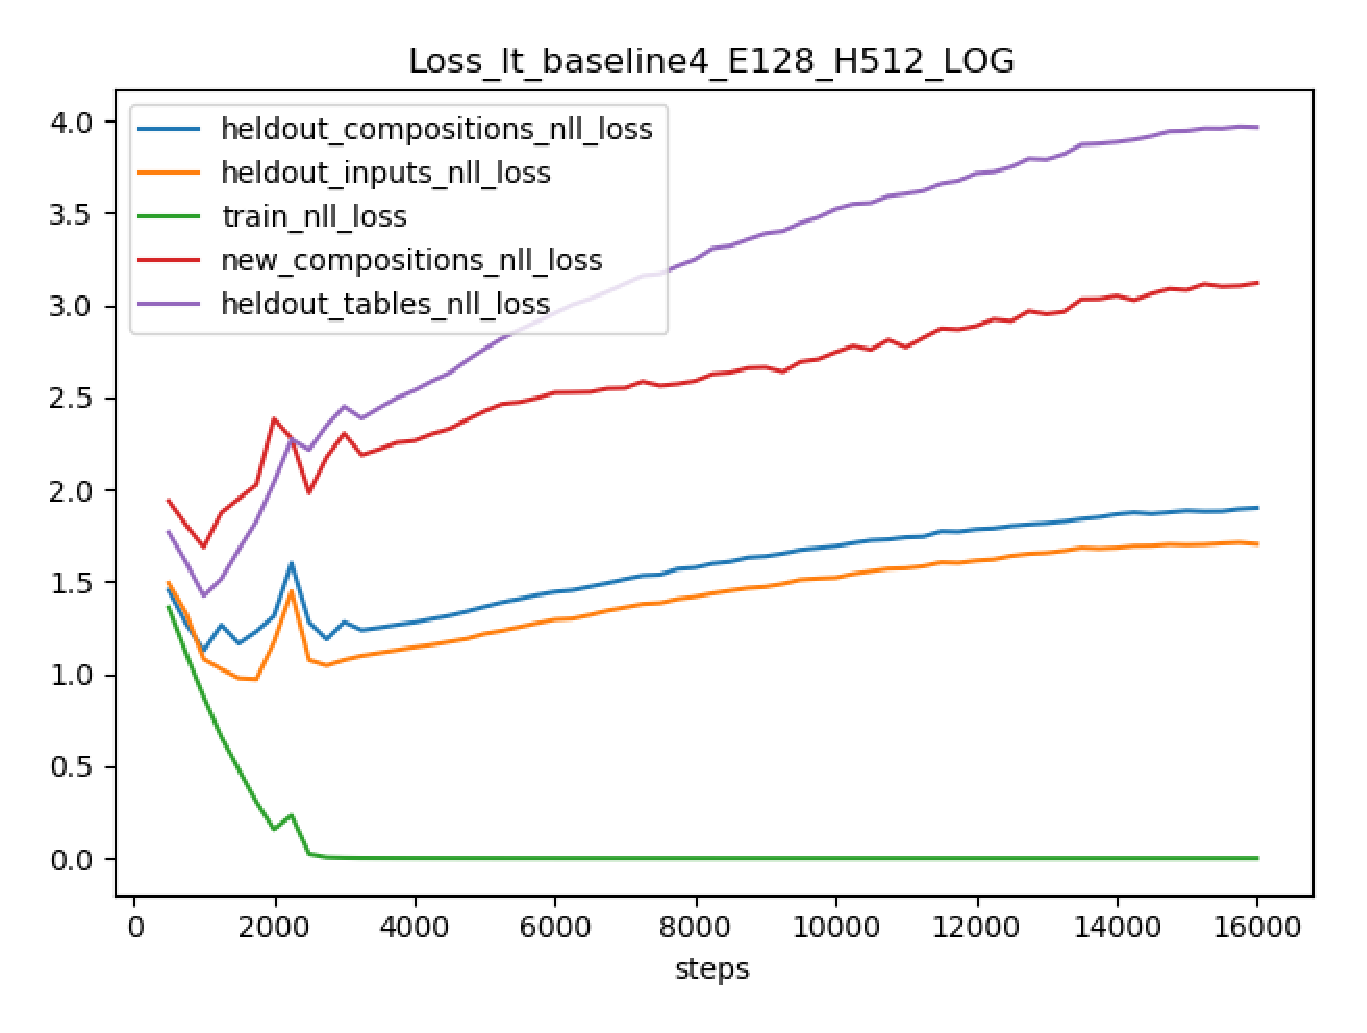
\includegraphics[width=0.95\linewidth]{./figs/lookup/baseline-loss-eps}
		\fi
		\caption{Loss Curves for Baseline} 
		\label{lt_baseline} 
		\vspace{2ex}
	\end{subfigure}%% 
	\begin{subfigure}[b]{0.5\linewidth}
		\centering
		\ifpdf
		\includegraphics[width=0.95\linewidth]{./figs/lookup/learned-loss-pdf}
		\else
		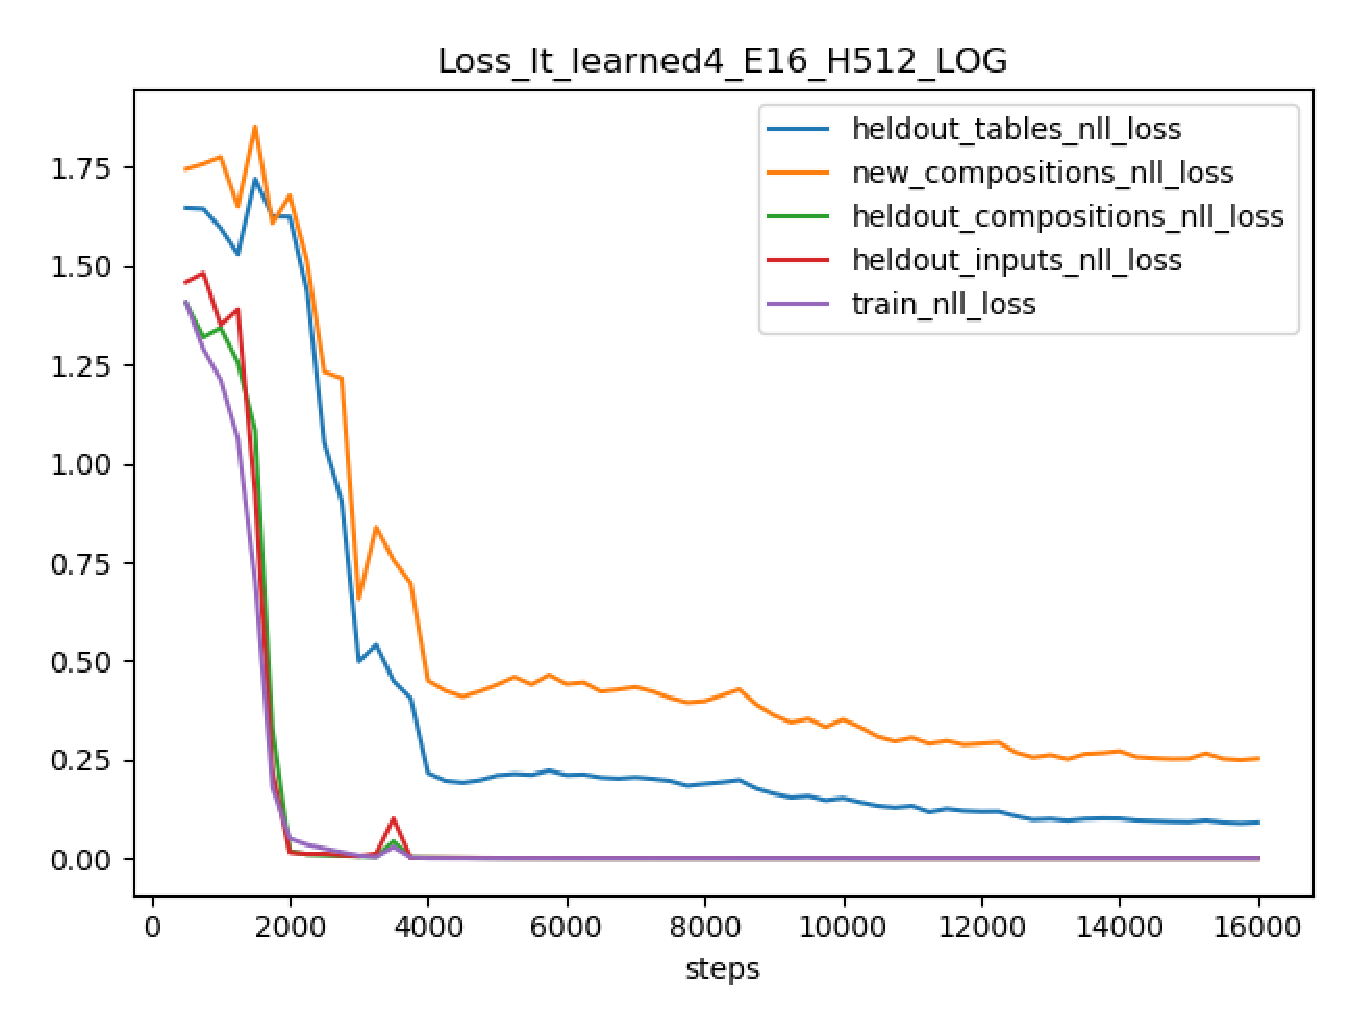
\includegraphics[width=0.95\linewidth]{./figs/lookup/learned-loss-eps}
		\fi 
		\caption{Loss Curves for Learned} 
		\label{lt_learned} 
		\vspace{2ex}
	\end{subfigure}
	\caption{Learning Curves for Lookup Tables}
	\label{lt_learning_curves}
\end{figure}

\begin{figure}
	\begin{minipage}[t]{0.9\textwidth}
		\centering
		\ifpdf
		\includegraphics[width=\linewidth,keepaspectratio=true]{./figs/lookup/lt-acc-pdf}
		\else
		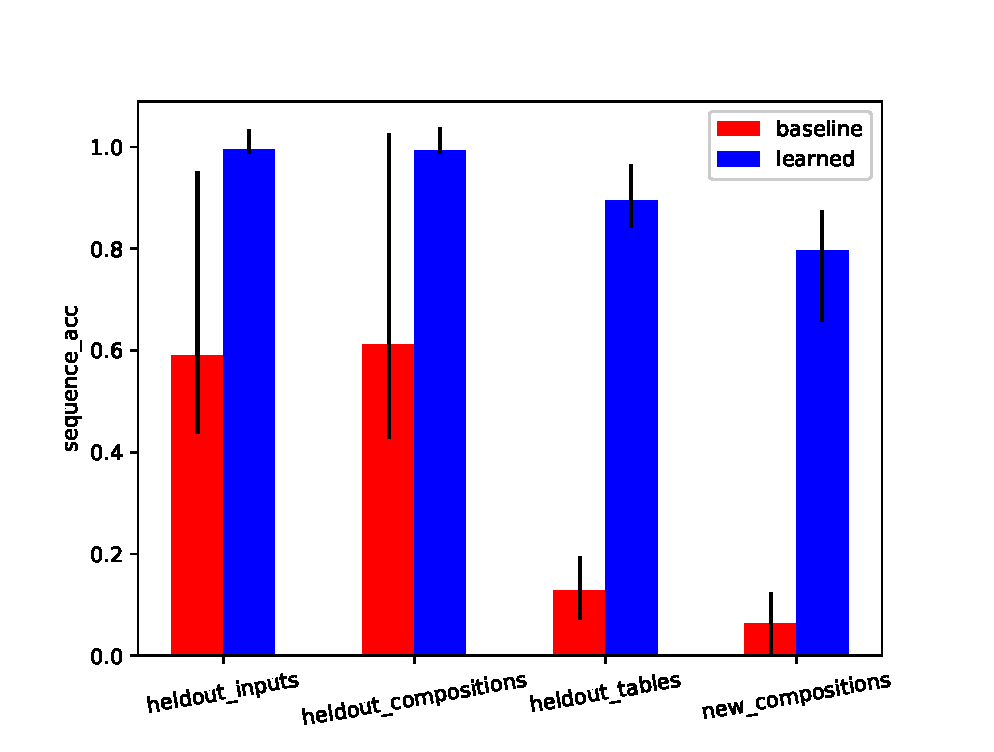
\includegraphics[width=\linewidth,keepaspectratio=true]{./figs/lookup/lt-acc-eps}
		\fi
		\caption{\small Average Sequence Accuracies}
		\label{res:lt-acc}
	\end{minipage}
\end{figure}

\begin{figure}[ht] 
	\begin{subfigure}[b]{0.5\linewidth}
		\centering
		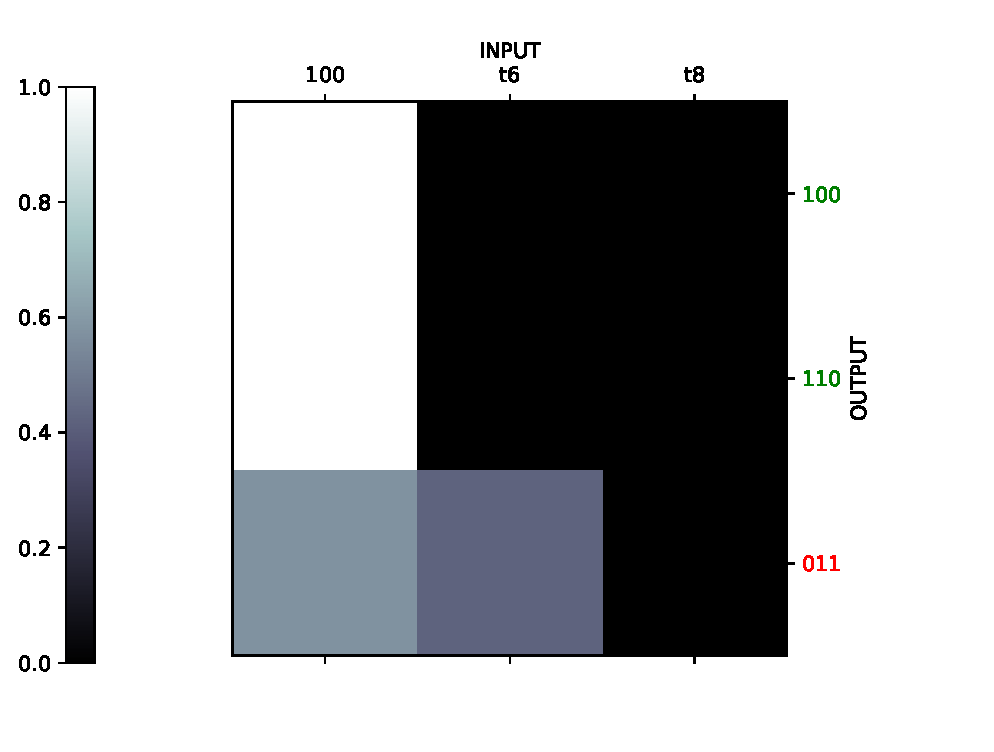
\includegraphics[width=0.95\linewidth]{./figs/lookup/attn/baseline1-eps}
		\caption{Heldout Tables} 
		\label{bs_attn1} 
		\vspace{2ex}
	\end{subfigure}%% 
	\begin{subfigure}[b]{0.5\linewidth}
		\centering
		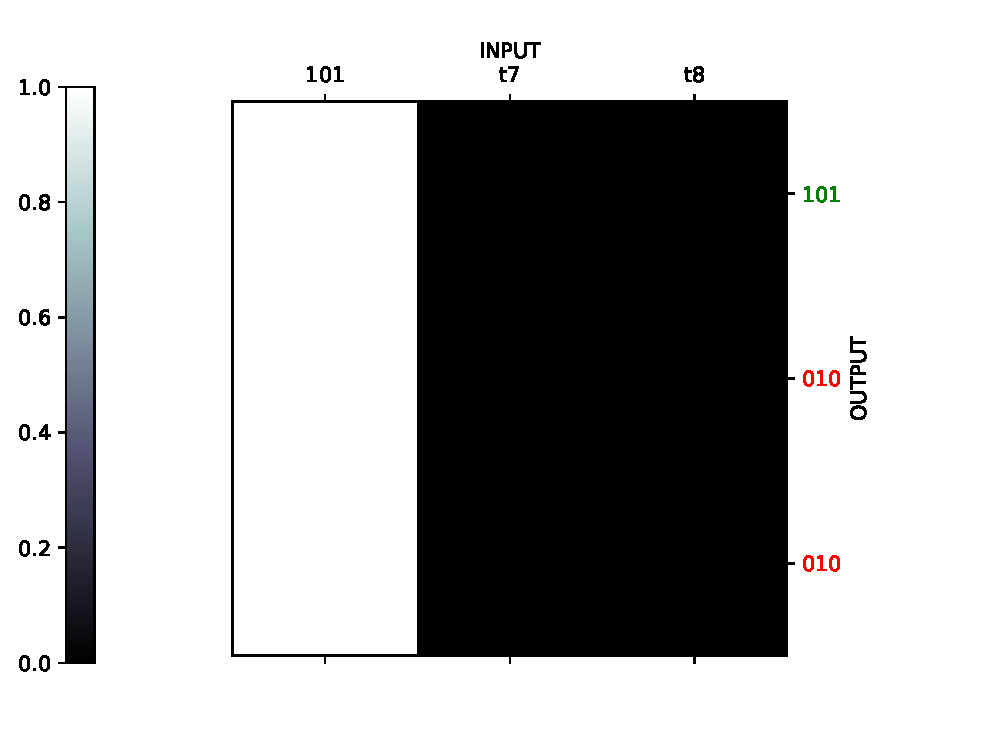
\includegraphics[width=0.95\linewidth]{./figs/lookup/attn/baseline2-eps}
		\caption{New Compositions} 
		\label{bs_attn2} 
		\vspace{2ex}
	\end{subfigure}
	\caption{Attention plots for baseline model.}
	\label{bs_attn}
\end{figure}

\begin{figure}[ht] 
	\begin{subfigure}[b]{0.5\linewidth}
		\centering
		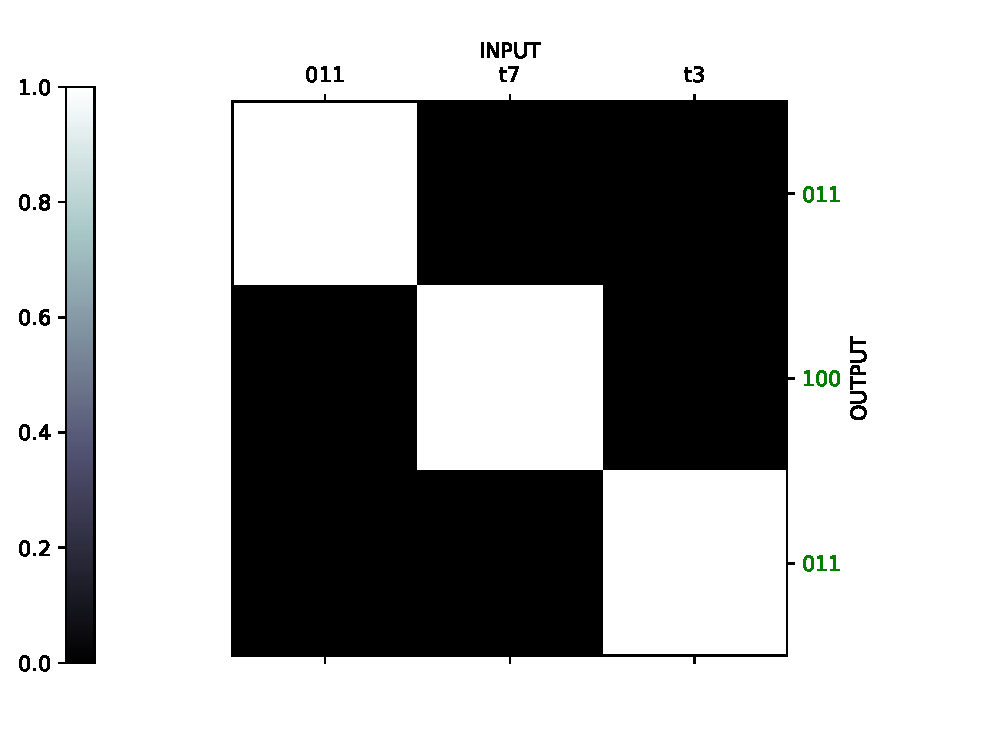
\includegraphics[width=0.95\linewidth]{./figs/lookup/attn/learned1-eps}
		\caption{Heldout Tables} 
		\label{lrn_attn1} 
		\vspace{2ex}
	\end{subfigure}%% 
	\begin{subfigure}[b]{0.5\linewidth}
		\centering
		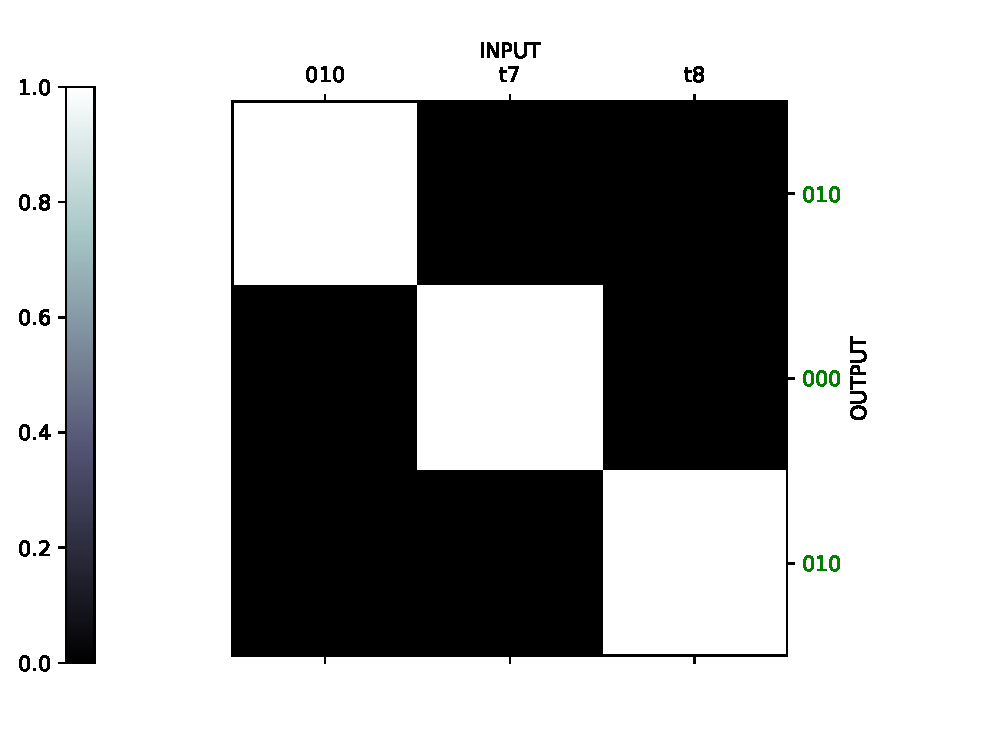
\includegraphics[width=0.95\linewidth]{./figs/lookup/attn/learned2-eps}
		\caption{New Compositions} 
		\label{lrn_attn2} 
		\vspace{2ex}
	\end{subfigure}
	\caption{Attention plot for guided model.}
	\label{lrn_attn}
\end{figure}


\begin{figure}[ht] 
	\begin{subfigure}[b]{0.5\linewidth}
		\centering
		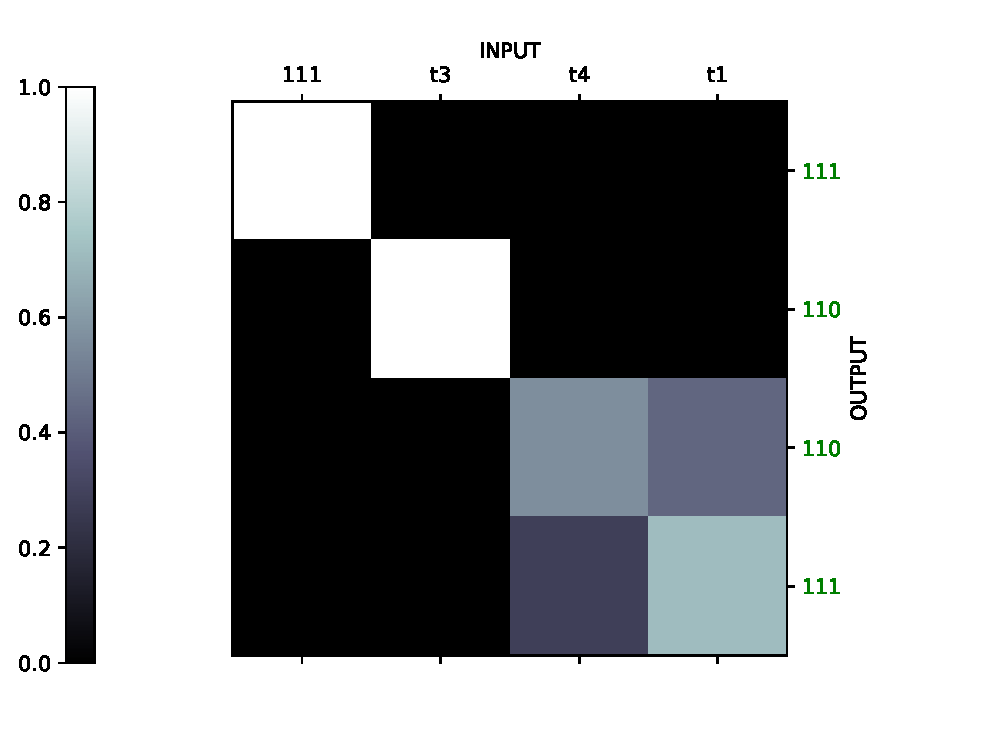
\includegraphics[width=0.95\linewidth]{./figs/lookup/attn/longer2-eps}
		\caption{Attention plot for length=3 heldout composition} 
		\label{attn_longer1} 
		\vspace{2ex}
	\end{subfigure}%% 
	\begin{subfigure}[b]{0.5\linewidth}
		\centering
		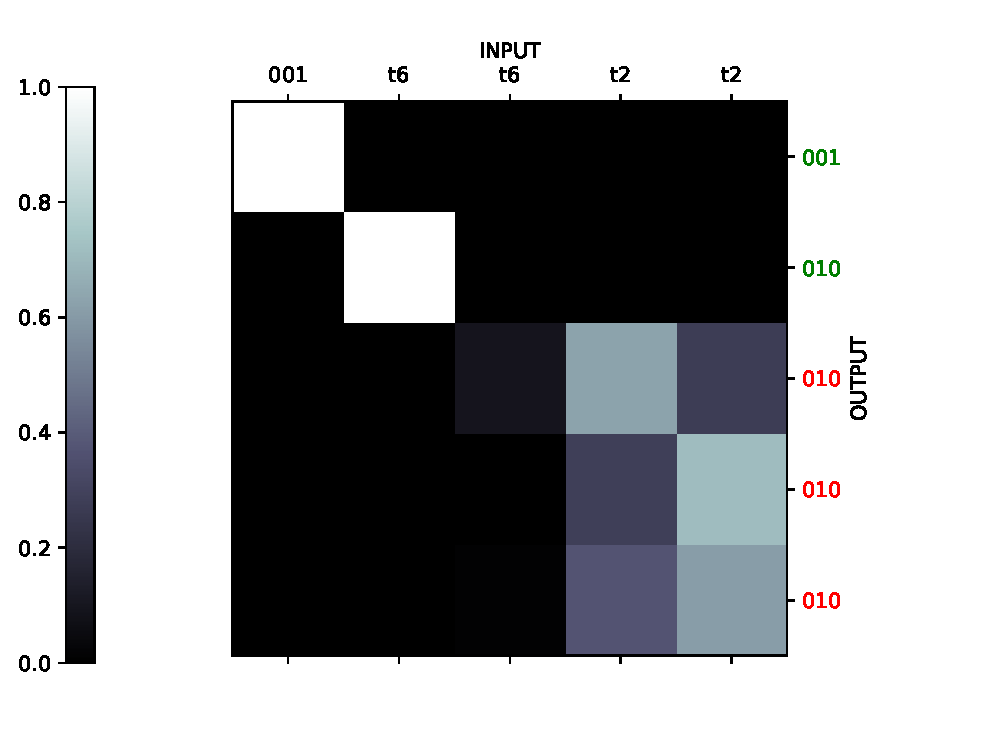
\includegraphics[width=0.95\linewidth]{./figs/lookup/attn/longer1-eps}
		\caption{Attention plot for length = 4 heldout composition} 
		\label{attn_longer2} 
		\vspace{2ex}
	\end{subfigure}
	\caption{Attention plot for longer heldout composition processed by a guided model.}
	\label{attn_longer}
\end{figure}

\begin{figure}[ht] 
	\begin{subfigure}[b]{0.5\linewidth}
		\centering
		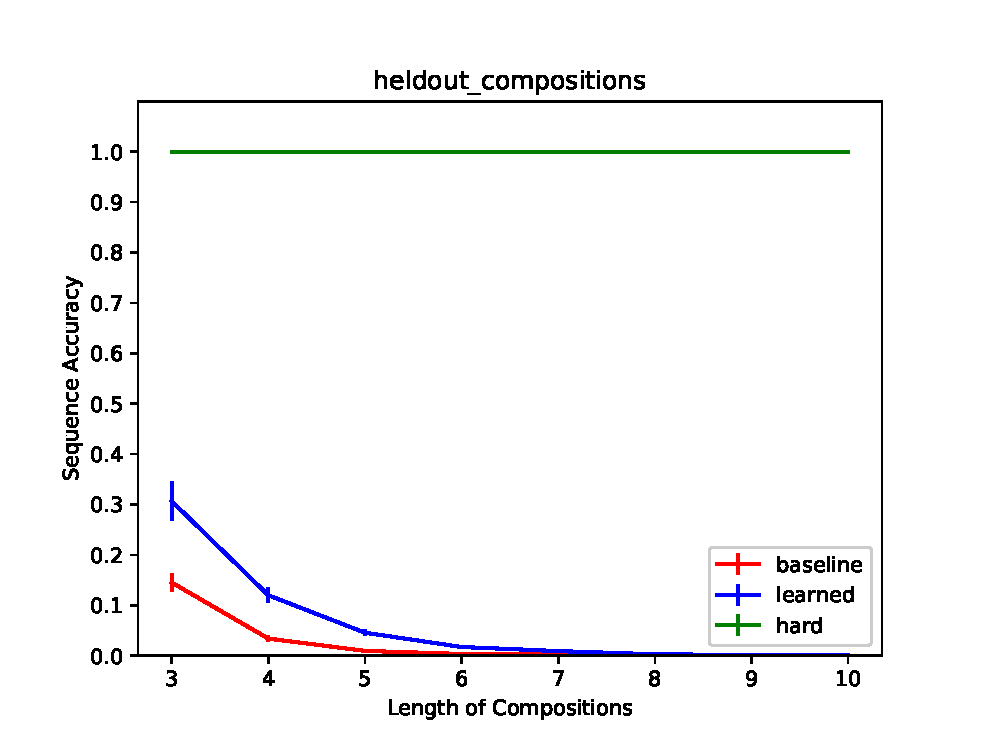
\includegraphics[width=0.95\linewidth]{./figs/lookup/heldout_compositions_eps}
		\caption{Longer Heldout Compositions} 
		\label{lt_longer1} 
		\vspace{2ex}
	\end{subfigure}%% 
	\begin{subfigure}[b]{0.5\linewidth}
		\centering
		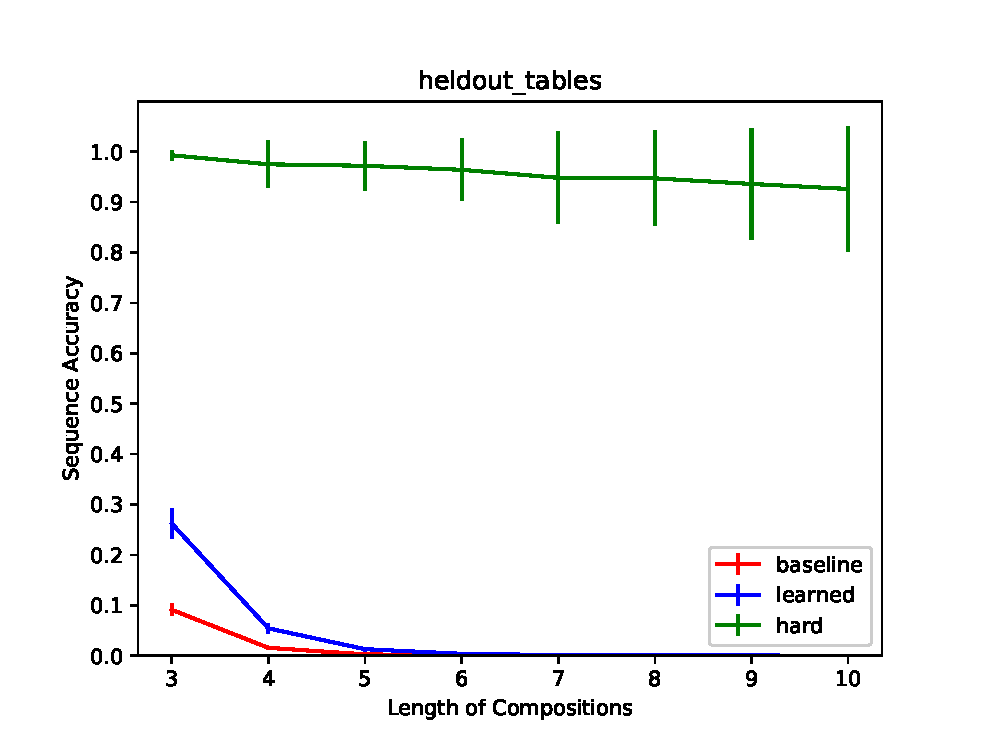
\includegraphics[width=0.95\linewidth]{./figs/lookup/heldout_tables_eps}
		\caption{Longer Heldout Tables} 
		\label{lt_longer2} 
		\vspace{2ex}
	\end{subfigure}
	\caption{Sequence Accuracy for Longer Compositions}
	\label{lt_longer}
\end{figure}



\section{Symbol Rewriting} \label{datasets:sr}
Introduced by \cite{Weber2018} the symbol rewriting dataset is essentially a probabilistic context free grammar (PCFG). It consists of a rewriting a set of input symbols to a set of output symbols based on this grammar. Before proceeding further with the task description,I'll elaborate on PCGFs briefly.

\subparagraph{PCFGs} are the stochastic version of CFGs (Context free grammars) that we encountered in section \ref{flt:ch}. The addition of this stochasticity was motivated by the non-uniformity of words in natural language. Assigning probabilities to production rules, lead to a grammar more in line with the Zipfian distribution of words in natural language \citep{jurafsky2014speech}. A PCFG consists of:

\begin{enumerate}
	\item A CFG $\mathcal{G} = \langle \Sigma, N, S, R \rangle$ where the symbols have the same meaning as defined in section \ref{flt}.
	\item A probability parameter $p(a \rightarrow b) \mid \displaystyle \sum_{a \rightarrow b \mid a \in N} p(a \rightarrow b) = 1 $ 
	\item $\therefore$ the probabilities associated with all the expansion rules of a given non-terminal should sum up to 1.
\end{enumerate}

\begin{figure}
	\begin{minipage}[ht]{\textwidth}
		\ifpdf
		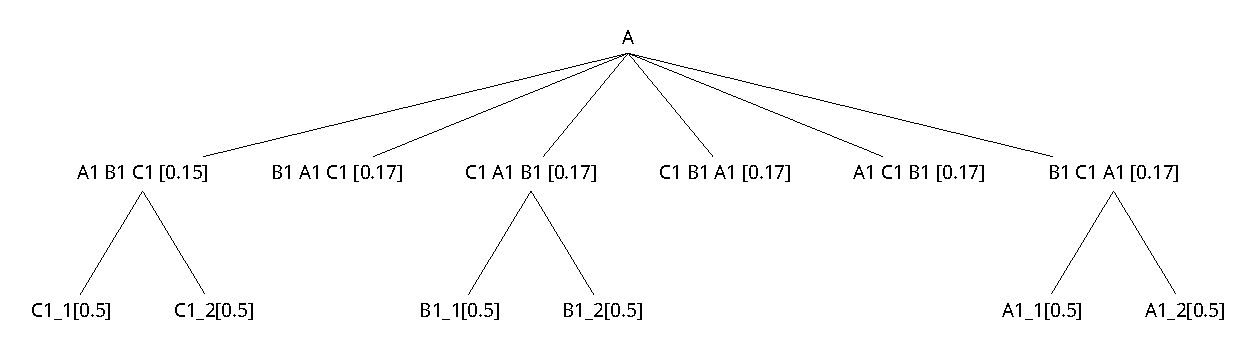
\includegraphics[width=\linewidth,keepaspectratio=true]{./figs/A-pdf}
		\else
		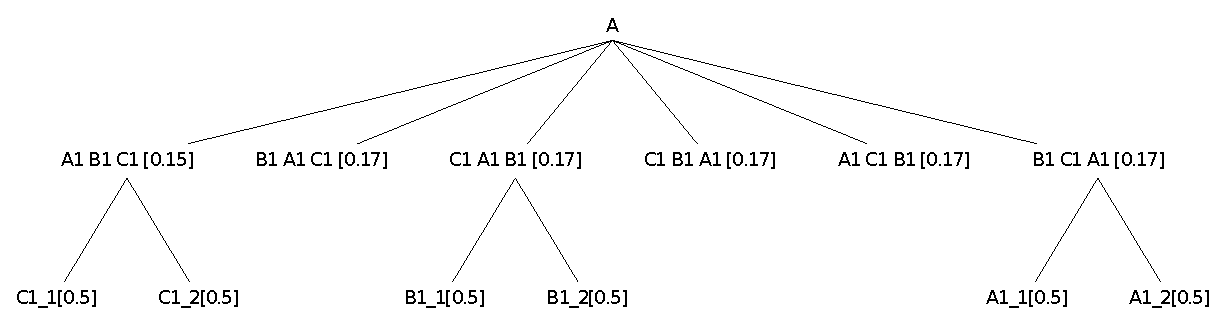
\includegraphics[width=\linewidth,keepaspectratio=true]{./figs/A-eps}
		\fi
		\caption{\small Parse Tree for one Input Symbol. The final symbols (leaf nodes) are shown just once with respect to their parent nodes for clarity.}
		\label{parse-tree}
	\end{minipage}
\end{figure}

The parse tree shown in figure \ref{parse-tree} illustrates the production rule for one input symbol. The grammar consists of 40 such symbols each following similar production rules. \cite{Weber2018} showed using this dataset while seq2seq models are powerful enough to learn some structure from this data and generalize on a test set which was drawn from the same distribution as the training set. They posit that given the simplicity of the grammar it should be possible to generalize to test sets (with some hyperparameter tuning) that are atypical of the training distribution while still conforming to the underlying grammar. They however show that this indeed \textbf{is not} the case.

\subsection{Data Structure}
The data-splits as furnished \citep{Weber2018} consists of a training data and different test cases which are non-exhaustive and created by sampling randomly from all possible i/o pairs as described by the PCFG. The different test sets are created to ascertain if the seq2seq models actually understand the underlying grammar from the training data or simply memorize some spurious structure from the training distribution. For hyperparameter tuning a validation set which is an amalgamation of random samples from all the different test sets, is used. The details of the different data splits are presented below. Examples from each split and the size of each split are presented in table \ref{sr:stats}
\begin{enumerate}
	\item \textbf{train} consists of 100000 pairs of input output symbols with input string length ranging between $\langle$ 5 and 10 $\rangle$. Output string length is therefore between $\langle$ 15 and 30 $\rangle$. A crucial feature of this set is that no symbol is repeated in a given input string.
	\item \textbf{standard test} consists of samples drawn from the same distribution as the training set.
	\item \textbf{repeat test} includes input strings where repetition of symbols is allowed.
	\item \textbf{short test} includes input strings which are shorter in length as compared to the input strings in the training data. The input string length ranges between $\langle$ 1 and 4 $\rangle$.
	\item \textbf{long test} consists of input sequences of lengths in the range $\langle$ 11 and 15 $\rangle$.
\end{enumerate}

\begin{table}[ht]
	\centering
	\begin{tabular}{l|lc}
		& Example & Size\\
		\hline
		train & HS E I G DS  & 100000 \\
		standard test & LS KS G E C P T & 2000 \\
		repeat & I I I I I I MS & 2000 \\
		short & M I C & 2000 \\
		long & Y W G Q V I FS GS C JS R B E M KS & 2000 \\
	\end{tabular}
	\caption{Symbol Rewriting Splits}
	\label{sr:stats}
\end{table}

The datasets \textit{repeat, short and long} come from distributions which are different from the training distribution on which the model has learned the data structure. It is expected of a compositional learner that given the sufficient size of the training data it would be able to infer a pattern which is close to the underlying PCFG and therefore generalize of the test sets which comes from different distributions but have the same underlying structure.

\subsection{AG Trace}
Every input symbol leads to three emissions in the output sequence and each output symbol is generated by exactly one input symbol. Therefore for every emission in the output sequence the index of the input symbol responsible for the emission, is the trace. For every input there are three decoding steps and for all the three steps the decoder should attend to that particular input.


\subsection{Accuracy}
Given the probabilistic nature of the symbol rewriting dataset it is not difficult to reason that sequence accuracy wouldn't be the ideal performance metric for this task. For instance A $\rightarrow$ A1\_1 B1\_2 C1\_1 and A $\rightarrow$ A1\_2 B1\_1 C1\_2 are both valid productions and since the data is probabilistic, the possibility of both the targets in the training data is equally likely. The accuracy of a prediction is evaluated in the following three steps:
\begin{itemize}
	\item Since every input symbol leads to emission of three output symbols, the output length should be 3*input length.
	\item The input vocabulary consists of 40 symbols (A - OS). The output is always a permutation of a three tuple of the form (Aj\_i Bj\_i Cj\_i) with $j=$ index of the corresponding input symbol in the vocabulary and $i \in [1, 2] $. The second check is to ensure that none of the Aj\_i Bj\_i Cj\_i are repeated.
	\item The third check is that the $j$ as described above = index of the corresponding input symbol in the vocabulary.
\end{itemize}
If a prediction passes all these three checks in that order, the accuracy of that prediction is 1 else 0.

\subparagraph{Hyperparameters}

\subsection{Symbol Rewriting - Results}

\begin{figure}
	\begin{minipage}[t]{0.9\textwidth}
		\centering
		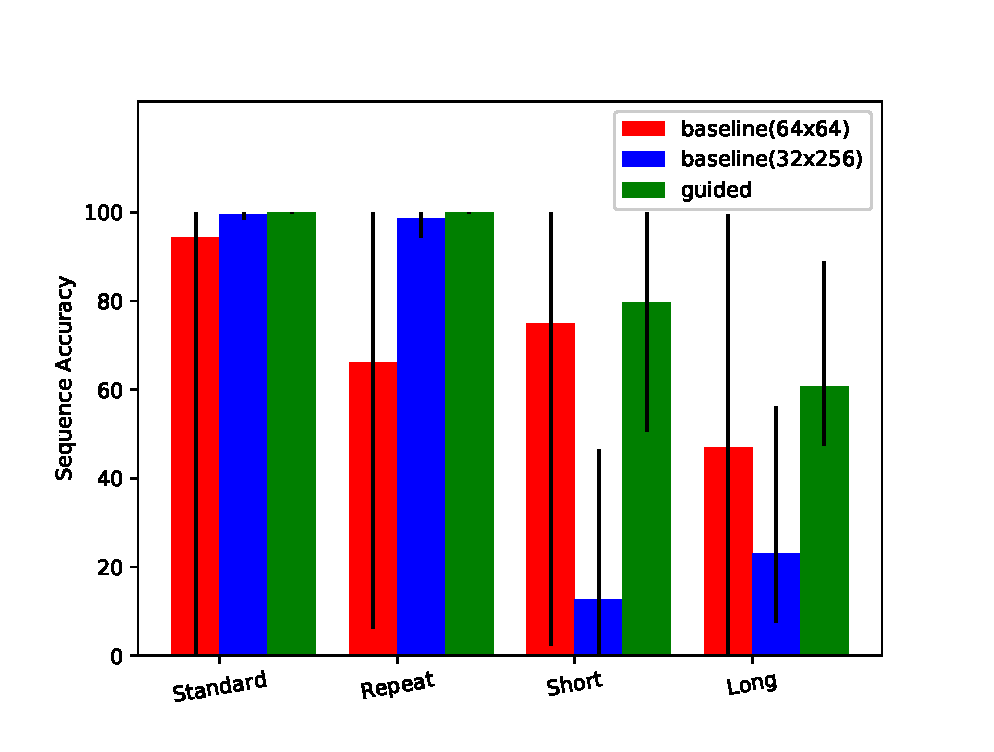
\includegraphics[width=\linewidth,keepaspectratio=true]{./figs/sr/sr-seq-eps}
		\caption{\small Sequence accuracies for symbol rewriting test splits}
		\label{res:sr-acc}
	\end{minipage}
\end{figure}

\begin{figure}[ht] 
	\begin{subfigure}[b]{0.5\linewidth}
		\centering
		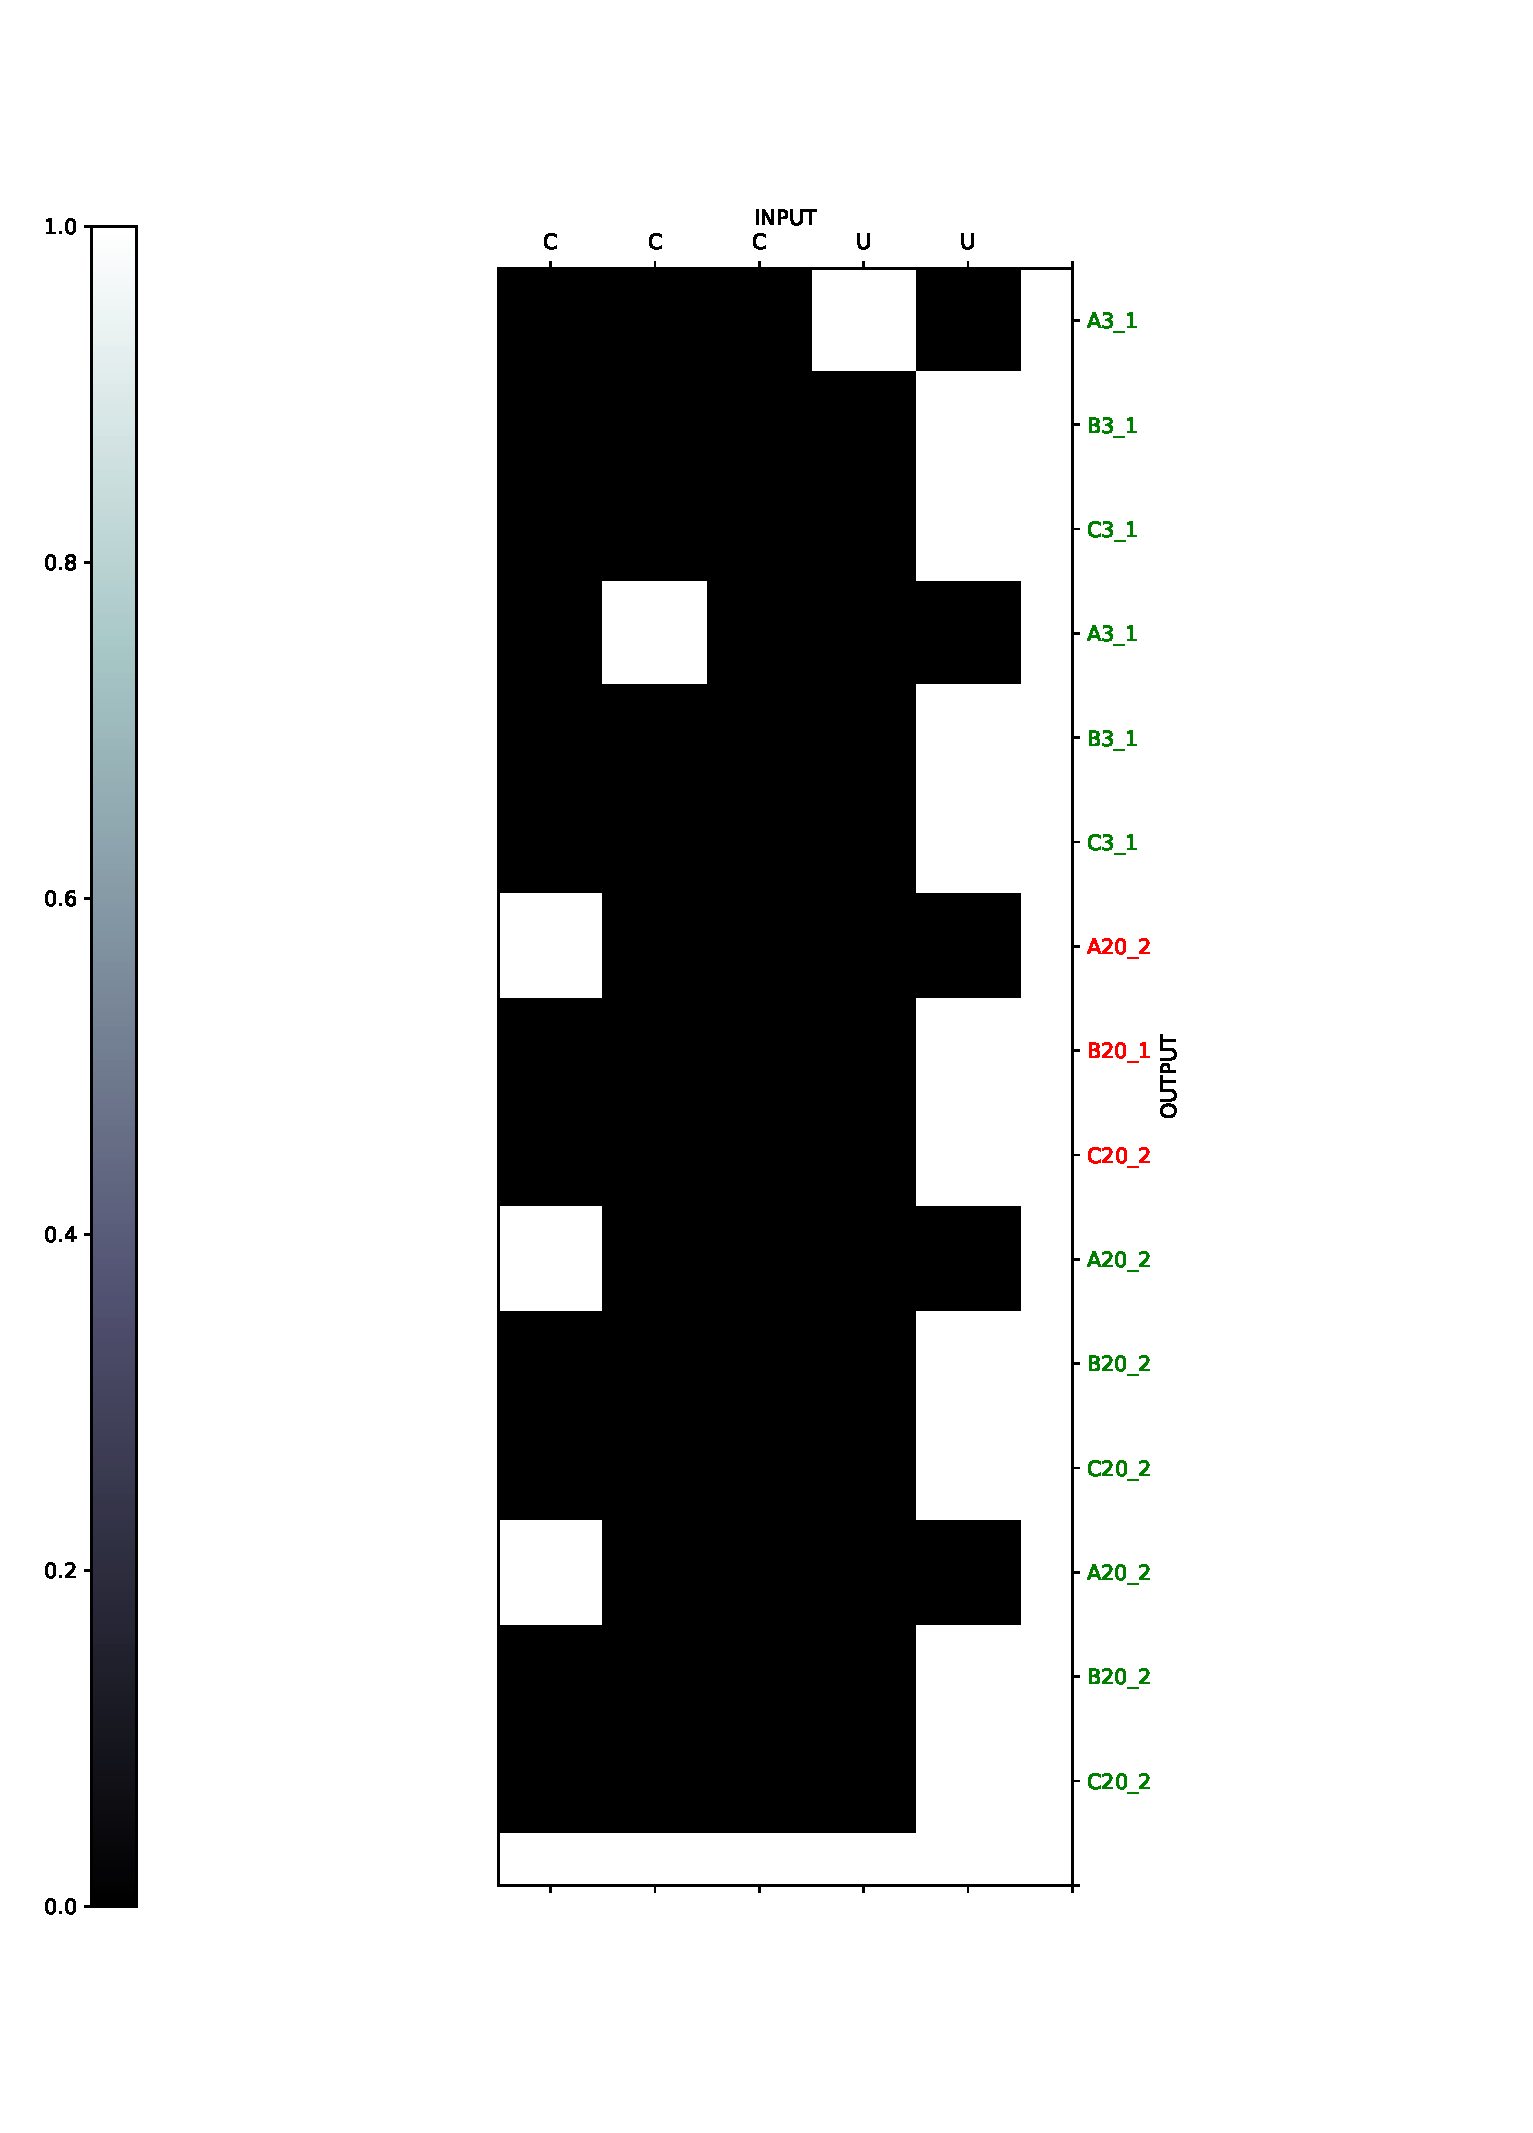
\includegraphics[width=0.95\linewidth]{./figs/sr/attn/baseline-eps}
		\caption{Baseline attention plot for a \lq repeat\rq{} sample} 
		\label{repeat_base} 
		\vspace{2ex}
	\end{subfigure}%% 
	\begin{subfigure}[b]{0.5\linewidth}
		\centering
		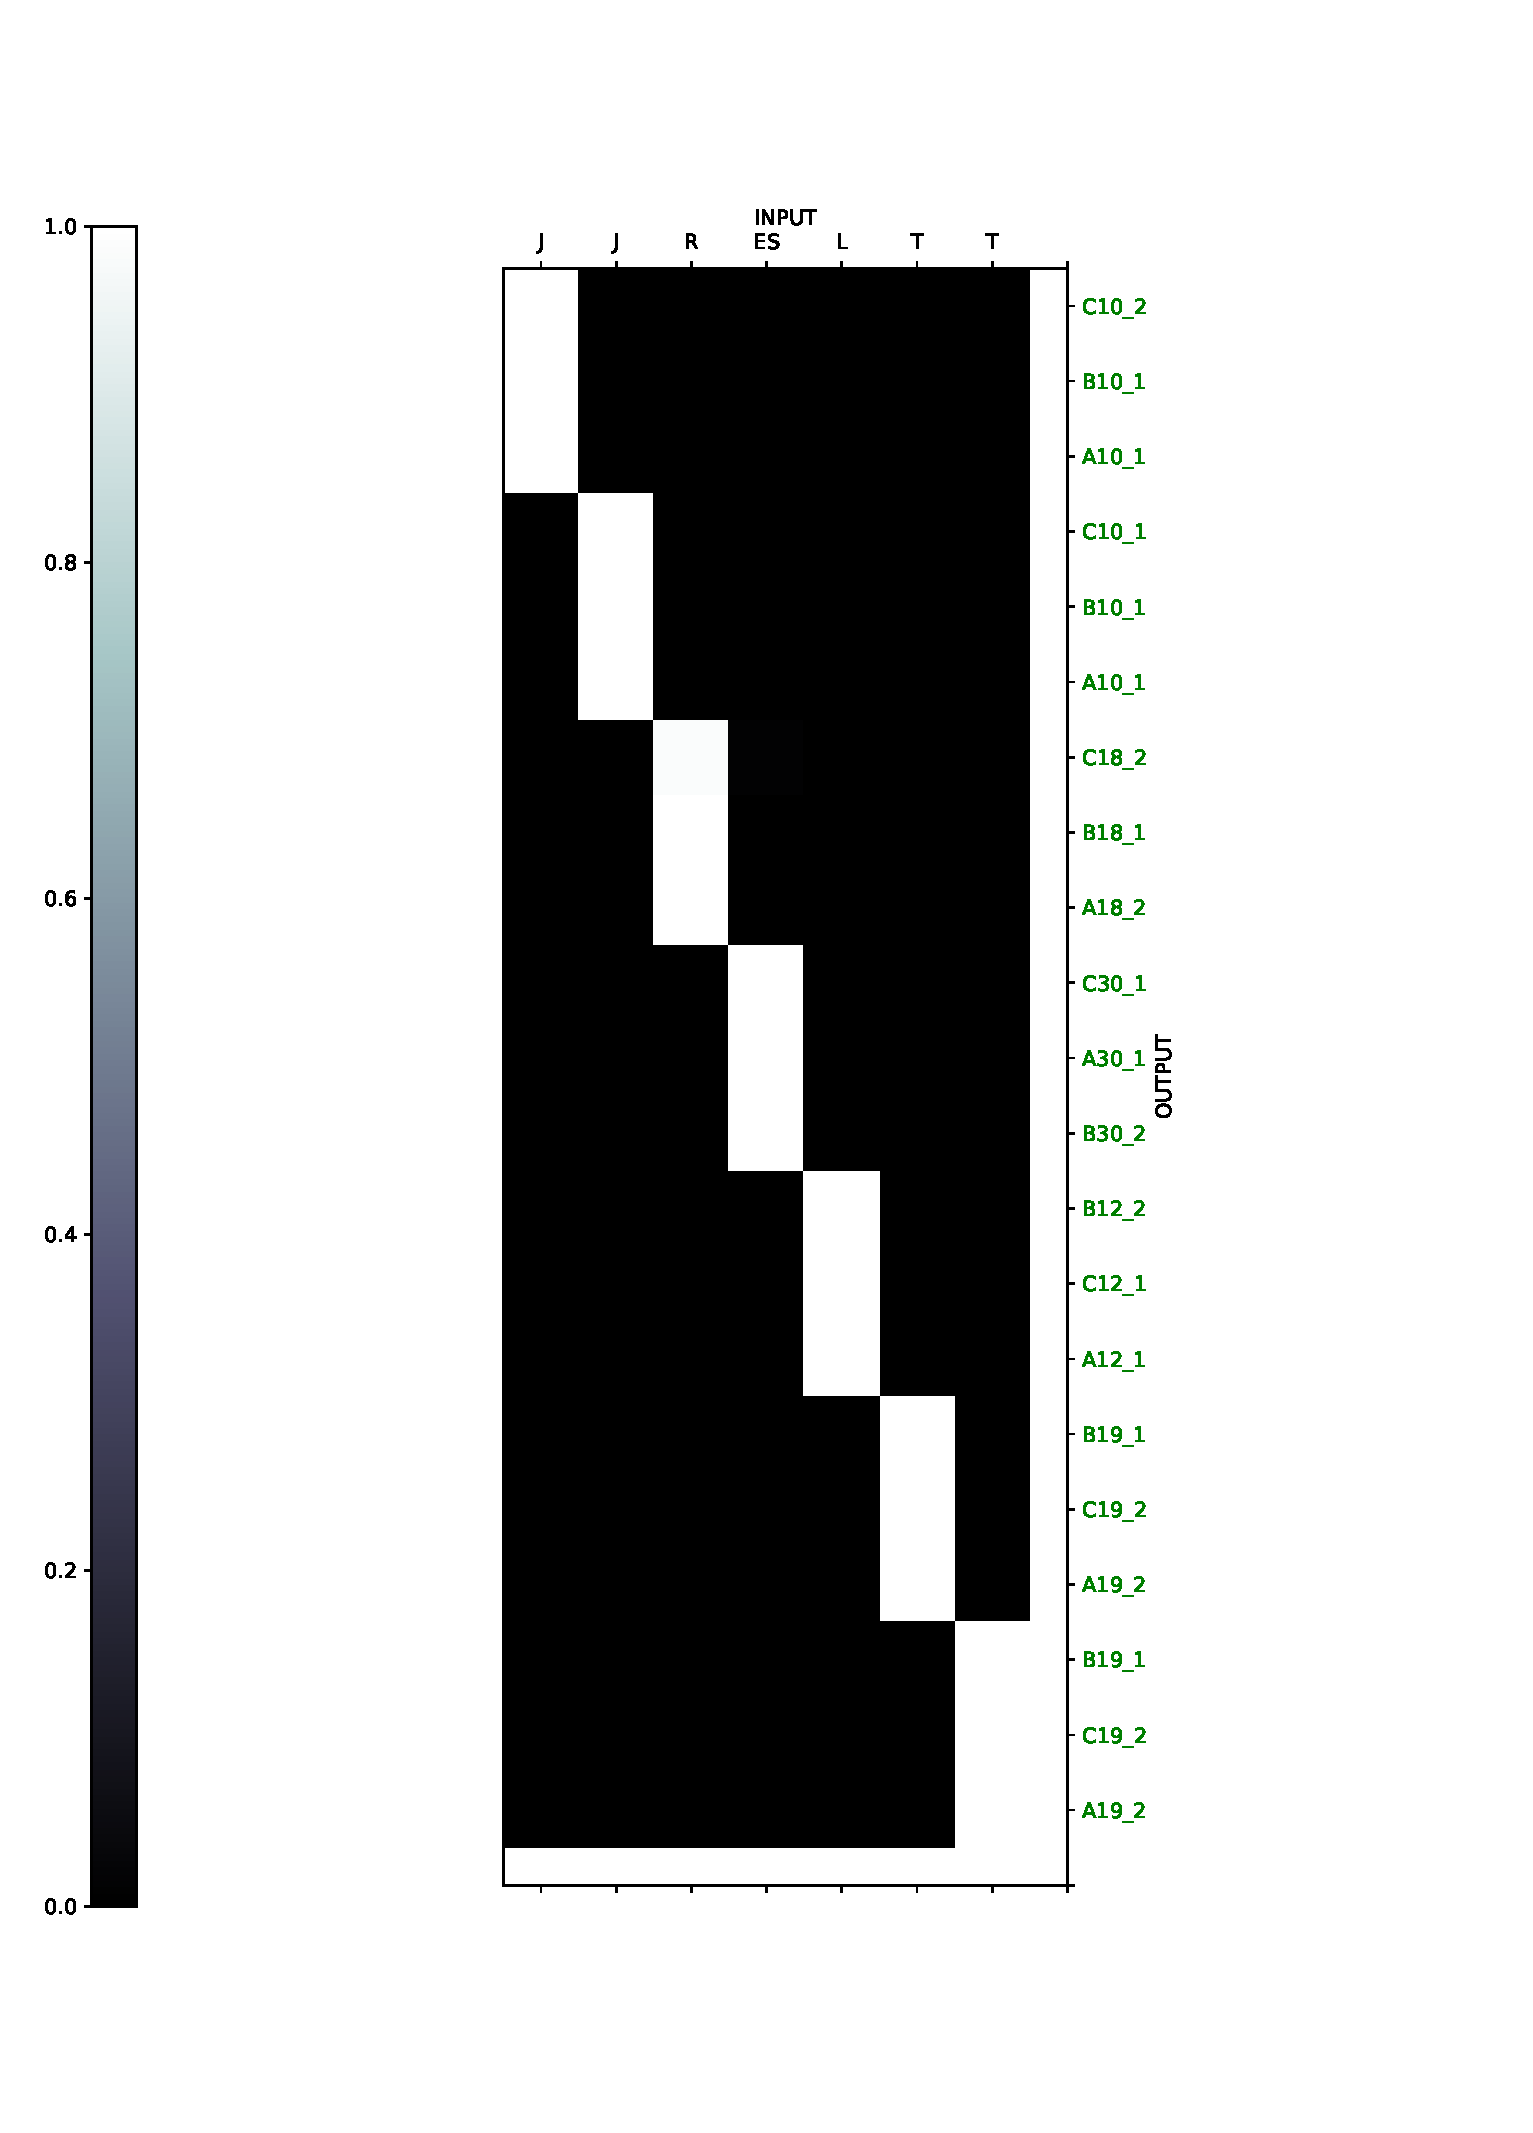
\includegraphics[width=0.95\linewidth]{./figs/sr/attn/guided-eps}
		\caption{AG attention plot for a \lq repeat\rq{} sample } 
		\label{repeat_guide} 
		\vspace{2ex}
	\end{subfigure}
	\caption{Attention plots for symbol rewriting}
	\label{sr_repeat}
\end{figure}
